\chapter{Contents of the Attached Memory Media}
\label{appendix-media}
This appendix describes the contents of the attached memory media. The memory media contains:
\begin{itemize}
    \item \texttt{d2a/} -- the original D2A dataset, which can also be downloaded from~\cite{D2A-webpage}.
    \item \texttt{d2a-bitcode/} -- zipped LLVM bitcode for the httpd project -- only for testing the generation of Graph D2A, so that LLVM bitcode does not have to be re-generated (it is computationally expensive).
    \item \texttt{d2a-filtered/} -- filtered D2A dataset.
    \item \texttt{graph-d2a/} -- zipped Graph D2A (raw ECPGs) for all projects from which TFRecords were generated, namely httpd, libtiff, nginx, and libav (the latter is divided into several parts as detailed below). So far, it has not been possible to find a place for online storage of the entire D2A Graph, which occupies hundreds of GBs when compressed. Once the D2A Graph is uploaded, a link will be provided in the \texttt{README.md} of the repository.
    \item \texttt{httpd-dependencies/} -- already configured libraries necessary for generating LLVM bitcode for httpd.
    
    \item \texttt{repository/} -- all the source files, which are also available on GitHub\footnote{GitHub repository: \url{https://github.com/TomasBeranek/but-masters-thesis}.}
    \begin{itemize}
        \item \texttt{dataset/} -- source files for the D2A to Graph D2A transformation.
        \begin{itemize}
            \item \texttt{construction\_phase\_d2a} -- for generating Graph D2A, see Section~\ref{implementation-graph-construction}.
            \item \texttt{filter.py} -- for filtering D2A, see Section~\ref{implementation-d2a-filter}.
            \item \texttt{generate\_bitcode.py} -- for generating LLVM bitcode, see Section~\ref{implementation-bitcode-generator}
            \item \texttt{Makefile} -- for automating the execution of these scripts.
        \end{itemize}
        \item \texttt{dev-utils/} -- a set of scripts that do not belong to the main implementation but were used, for example, for data exploration and other useful tasks.
        \begin{itemize}
            \item \texttt{concat\_tfrecords.py} -- for concatenating TFRecords files.
            \item \texttt{extract\_sample.py} -- for extracting and displaying samples from D2A.
            \item \texttt{find\_unique\_values.py} -- for finding unique attribute values in Graph D2A.
            \item \texttt{graphs\_comparison.sh} -- for comparing different  versions of Graph D2A.
            \item \texttt{records\_counter.py} -- for counting samples in TFRecords files.
            \item \texttt{remove\_duplicates.py} -- for removing duplicate samples in D2A at the LLVM bitcode level.
            \item \texttt{remove\_invalid\_symlinks.py} -- for removing incorrect symlinks in LLVM bitcode (this issue has been fixed).
            \item \texttt{stats.py} -- for generating statistics about D2A -- Tables~\ref{tab:d2a-bug-types1} and~\ref{tab:d2a-bug-types2}.
        \end{itemize}
        \item \texttt{experiments/} -- a set of experiments that support and demonstrate various claims made in this thesis. If an experiment is executable, it can be run using the \texttt{make} command in its directory. Details of the experiment are provided for each experiment separately (typically in \texttt{Makefile}). 
        \begin{itemize}
            \item \texttt{arg-passing/} -- demonstration of argument passing in raw ECPG.
            \item \texttt{comparison-with-chatgpt/} -- data for comparison with ChatGPT, from Section~\ref{comparison-chatgpt}.
            \item \texttt{compilation-from-D2A/} -- demonstration that code cannot be compiled directly from D2A.
            \item \texttt{entry-function/} -- demonstration that Infer always reports the entry function in the \texttt{procedure} attribute.
            \item \texttt{global-vars/} -- demonstration of storing access to global variables in raw ECPG.
            \item \texttt{include-headers-to-bitcode/} -- demonstration that slicing criteria can also be specified for \texttt{.h} files because they are included in LLVM bitcode.
            \item \texttt{joern-batch-processing/} -- demonstration that Joern batch processing is equivalent to single sample processing.
            \item \texttt{line-slicing/} -- demonstration that LLVM slicer retains everything on the line specified as the slicing criterion.
            \item \texttt{removing-duplicates/} -- test to demonstrate the functionality of removing duplicate samples.
            \item \texttt{speed-test/} -- comparison of repository search types by speed when generating LLVM bitcode.
            \item \texttt{struct-alias/} -- demonstration of storing structures and aliases in raw ECPG.
        \end{itemize}
        \item \texttt{inference-pipeline/} -- source code of the inference pipeline.
        \begin{itemize}
            \item \texttt{example/} -- an artificial example to demonstrate the functionality of the inference pipeline.
            \item \texttt{inference\_pipeline} -- inference pipeline, see Section~\ref{implementation-inference-pipeline}.
            \item \texttt{Makefile} -- for installing/uninstalling compiler wrappers and running the experiment.
            \item \texttt{model\_inference.py} -- for inference using GNN models, see Section~\ref{implementation-inference-pipeline}.
            \item \texttt{slicing\_criteria\_extraction.py} -- for extraction of slicing criteria, from Section~\ref{implementation-slicing-info}.
            \item \texttt{wrapper} -- template for compiler wrapper, see Section~\ref{implementation-compiler-wrapper}.
        \end{itemize}
        \item \texttt{model/} -- source files for feature engineering, training, and testing models.
        \begin{itemize}
            \item \texttt{schemas/} -- source files for feature engineering.
            \begin{itemize}
                \item \texttt{extended\_cpg.pbtxt} -- TFGNN schema for ECPG.
                \item \texttt{feature\_engineering.py} -- feature engineering, see Section~\ref{implementation-feature-engineering}.
                \item \texttt{find\_normalization\_coefficients.py} -- for extraction of normalization coefficients, see Section~\ref{implementation-norm-coeffs}.
                \item \texttt{Makefile} -- targets for automating the execution of these scripts.
            \end{itemize}
            \item \texttt{src/} -- source files for models.
            \begin{itemize}
                \item \texttt{evaluate\_model.py} -- for model evaluation, see Section~\ref{implementation-evaluation}.
                \item \texttt{mixed\_nodes\_model.py} -- for model training, see Section~\ref{implementation-training}.
            \end{itemize}
            \item \texttt{Makefile} -- targets for training models, evaluating models, and scenarios.
        \end{itemize}
        \item \texttt{sep-presentation-en/} -- \LaTeX\xspace source code of the SEP presentation.
        \item \texttt{sep-text-en/} -- \LaTeX\xspace source code of the SEP text.
        \item \texttt{text-en/} -- \LaTeX\xspace source code of this thesis.
        \item \texttt{text-template/} -- \LaTeX\xspace source code of the used template.
        \item \texttt{xberan46-2024.pdf} -- PDF version of this thesis.
        \item \texttt{.gitignore}
        \item \texttt{README.md}
    \end{itemize}

    \item \texttt{results/} -- output graphs for all scenarios from Section~\ref{implementation-evaluation}.
    \item \texttt{saved\_models/} -- all trained models -- \texttt{Model 1} to \texttt{Model 14}.
    \item \texttt{text-en/} -- \LaTeX\xspace source code of this thesis.
    \item \texttt{tfrecords/} -- dataset in TFRecords format for all projects that were used for training or testing, namely httpd, libtiff, nginx, and libav. The dataset in this format was also published on Zenodo \cite{zenodo-ecpg}.
    \item \texttt{xberan46-2024.pdf} -- PDF version of this thesis.
\end{itemize}



\chapter{Installation and User Manual}
\label{appendix-use-manual}
This appendix contains the installation and user manual, which were tested on a clean, normal (i.e., not minimal) installation of Ubuntu 20.04.2.0 LTS. For training or evaluating GNN models, it is advisable to have a GPU compatible with the TensorFlow library, otherwise the computation will be significantly slower.

\subsubsection{Installation}
All source code for training and inference pipelines is in script form, so there is no need for any installation, except for installing a compiler wrapper using a make target (see below). However, it is necessary to install required dependencies.

LLVM Slicer can be installed as follows\footnote{Official installation guide for LLVM Slicer:  \url{https://github.com/mchalupa/dg/blob/master/doc/compiling.md}.}:
\begin{lstlisting}[language=bash, xleftmargin=2em]
sudo apt install git cmake make llvm zlib1g-dev clang g++ python3.8
git clone https://github.com/mchalupa/dg
cd dg
mkdir build && cd build
cmake ..
make -j4
sudo ln -s ${PWD}/tools/llvm-slicer /usr/bin/llvm-slicer
\end{lstlisting}

Joern can be installed using:
\begin{lstlisting}[language=bash, xleftmargin=2em]
sudo apt install curl default-jdk default-jre
git clone https://github.com/joernio/joern
cd joern
sudo ./joern-install.sh
\end{lstlisting}

For LLVM2CPG, it is necessary to download the binary release for Ubuntu 20.04\footnote{LLVM2CPG's binary release for Ubuntu 20.04: \url{https://github.com/ShiftLeftSecurity/llvm2cpg/releases/download/0.8.0/llvm2cpg-0.8.0-LLVM-11.0-ubuntu-20.04.zip}.} and then install it using:
\begin{lstlisting}[language=bash, xleftmargin=2em]
unzip llvm2cpg-0.8.0-LLVM-11.0-ubuntu-20.04.zip
mv llvm2cpg-0.8.0-LLVM-11.0-ubuntu-20.04/ llvm2cpg
sudo ln -s ${PWD}/llvm2cpg/llvm2cpg /usr/bin/llvm2cpg
\end{lstlisting}

To generate LLVM bitcode, the following dependencies need to be installed for various projects:
\begin{itemize}
    \item httpd
\begin{lstlisting}[language=bash, xleftmargin=2em]
sudo apt install libpcre3 libpcre3-dev autoconf libtool-bin
\end{lstlisting}
    \item libtiff
\begin{lstlisting}[language=bash, xleftmargin=2em]
sudo apt install libgl-dev freeglut3-dev
\end{lstlisting}
    \item ffmpeg (the same applies to libav as they share some libraries)
\begin{lstlisting}[language=bash, xleftmargin=2em]
sudo apt install nasm yasm libsdl2-dev
\end{lstlisting}
    \item openssl
\begin{lstlisting}[language=bash, xleftmargin=2em]
sudo apt install perlbrew
perlbew init # follow the instructions to finish the installation
perlbrew install perl-5.28.0
\end{lstlisting}
\end{itemize}

It is also necessary to install Infer using the binary release\footnote{Infer's binary release: \url{https://github.com/facebook/infer/releases/download/v1.1.0/infer-linux64-v1.1.0.tar.xz}.}:
\begin{lstlisting}[language=bash, xleftmargin=2em]
tar xf infer-linux64-v1.1.0.tar.xz
sudo ln -s ${PWD}/infer-linux64-v1.1.0/bin/infer /usr/bin/infer
\end{lstlisting}

Additionally, the following Python3.8 packages must be installed:
\begin{lstlisting}[language=bash, xleftmargin=2em]
sudo apt install python3-pip
python3.8 -m pip install tqdm "pandas==1.3.4" "networkx==3.1" \
"matplotlib==3.4.3" "scikit-learn==1.2.0" "tensorflow-gnn==0.6.1"
\end{lstlisting}

The command line tool \texttt{parallel} also have to be installed:
\begin{lstlisting}[language=bash, xleftmargin=2em]
sudo apt install parallel
\end{lstlisting}

For experiments, the following dependencies are necessary:
\begin{lstlisting}[language=bash, xleftmargin=2em]
sudo apt install graphviz tree
\end{lstlisting}


\subsubsection{User Manual}
The training pipeline is divided into individual phases and is generated in parts due to its high computational demands. To simplify generation, a set of Makefiles has been created. However, using these Makefiles requires storing the individual outputs in directories exactly as defined below (or it is possible to modify the paths in the Makefiles, or call the tools without using Makefiles). The manual assumes that the starting working directory contains directories and files from the attached memory media.

The first step is to prepare D2A:
\begin{lstlisting}[language=bash, xleftmargin=2em]
mv d2a repository/dataset/
\end{lstlisting}

D2A is then filtered:
\begin{lstlisting}[language=bash, xleftmargin=2em]
cd repository/dataset/ && make filter-d2a
\end{lstlisting}

Next, the slicing criteria are extracted:
\begin{lstlisting}[language=bash, xleftmargin=2em]
make slicing-info
\end{lstlisting}

Then, prepare a directory for the repositories of individual projects from D2A, add pre-configured libraries for httpd (it is also possible to download from official sites and configure it as described in Section~\ref{implementation-bitcode-generator}), and download the original project repositories:
\begin{lstlisting}[language=bash, xleftmargin=2em]
mkdir projects && mv ../../httpd-dependencies projects/
make download-repos
\end{lstlisting}

From this point forward, commands will only be listed for the httpd project; other projects are generated similarly unless otherwise noted. LLVM bitcode is generated using:
\begin{lstlisting}[language=bash, xleftmargin=2em]
make bitcode-httpd-1
make bitcode-httpd-0
\end{lstlisting}

Before generating LLVM bitcode for openssl, it is necessary to switch the Perl version as follows:
\begin{lstlisting}[language=bash, xleftmargin=2em]
perlbrew switch perl-5.28.0
\end{lstlisting}

After generating the LLVM bitcode, it is possible to start generating the D2A Graph:
\begin{lstlisting}[language=bash, xleftmargin=2em]
mkdir -p graph-d2a/httpd_1 && make graph-httpd-1
mkdir -p graph-d2a/httpd_0 && make graph-httpd-0
\end{lstlisting}

The D2A Graphs for projects from which TFRecords were generated, namely httpd, libtiff, nginx, and libav, are zipped on the attached memory media in the \texttt{graph-d2a/} directory to avoid re-generation. Because the D2A Graph is not only computationally expensive to create but also memory-expensive to store, libav\_0 is split into 3 \texttt{.zip} files, which must be transformed into TFRecords separately, and the results combined using the script \texttt{repository/dev-utils/concat\_tfrecords.py} (an example of its usage is provided inside).

Normalization coefficients could be extracted here, but they have already been generated and are inserted directly in \texttt{feature\_engineering.py}. However, for demonstration, it can be done using:
\begin{lstlisting}[language=bash, xleftmargin=2em]
cd ../model/schemas && make extract-norm-coeffs-httpd
\end{lstlisting}

Extraction of normalization coefficients is also possible for libtiff and nginx. For other projects, make targets were not created as they were not used for training.

To generate TFRecords, enter (current working directory is \texttt{repository/model/schemas}):
\begin{lstlisting}[language=bash, xleftmargin=2em]
mkdir ../tfrecords
make transform-httpd-1
make transform-httpd-0
\end{lstlisting}

Once TFRecords for the httpd, libtiff, and nginx projects are created, training can commence. As their generation is also time-consuming, they are included on the memory media in the \texttt{tfrecords} directory, or are available on Zenodo \cite{zenodo-ecpg}. To start training the currently configured model (the architecture of \texttt{Model 8} -- the best standalone model) with combined data, along with adding \texttt{tfrecord} from the media and also adding models from the media (\texttt{saved\_models/}), use:
\begin{lstlisting}[language=bash, xleftmargin=2em]
cd ..
mv ../../tfrecords .
mv ../../saved_models . 
make train-combined-model
\end{lstlisting}

For example, \texttt{Model 8} can be evaluated on the test data using:
\begin{lstlisting}[language=bash, xleftmargin=2em]
make evaluate-model-test ID=8
\end{lstlisting}

Alternatively, it is possible to run, for example, a \texttt{combined} scenario:
\begin{lstlisting}[language=bash, xleftmargin=2em]
make scenario-combined
\end{lstlisting}

For a demonstration of the inference pipeline, a simple project was created in which Infer finds 3 errors -- 1x \texttt{DEAD\_STORE} (which is not supported as it is always true positive) and 2x \texttt{NULL\_DEREFERENCE}. When executing the experiment, compiler wrappers are first installed, the project is compiled, the inference pipeline is run, and finally, the wrappers are uninstalled. The experiment can be initiated (assuming the working directory is \texttt{repository/model/}):
\begin{lstlisting}[language=bash, xleftmargin=2em]
cd ../inference-pipeline
make
\end{lstlisting}

The output is \texttt{ranked\_report.json}, where errors are scored (attribute \texttt{model\_score}) and ranked using \texttt{Model 8}.


\chapter{Additional Data}
\label{appendix-additional-data}
This appendix contains supplementary tables and figures that provide additional data relevant to the discussions and experiments presented in earlier chapters of the thesis.

\begin{table}[ht]
    \centering
    \caption{The table contains the distribution of all D2A samples (except the after fix type) by error type and label (true positive/false positive). This table shows the distribution for the openssl, libav, and nginx projects. Table~\ref{tab:d2a-bug-types2} shows the distribution for the remaining projects. The green highlighted rows represent the types of errors supported by the system designed in this thesis.}
    \vskip6pt
    \begin{tabular}{!{\vrule width 1pt}l!{\vrule width 1pt}c|c|c!{\vrule width 1pt}c!{\vrule width 1pt}}
        \noalign{\hrule height 1pt}
         {\footnotesize\textbf{Error Type}} & {\footnotesize\textbf{openssl}} & {\footnotesize\textbf{libav}} & {\footnotesize\textbf{nginx}}\\
         \noalign{\hrule height 1pt}
         \rowcolor{green!20}
         {\scriptsize INTEGER\_OVERFLOW\_L5}&  {\footnotesize 4046/166221}&  {\footnotesize 2892/156942}&  {\footnotesize 162/4333}\\ \hline
         \rowcolor{green!20}
         {\scriptsize BUFFER\_OVERRUN\_L5}&    {\footnotesize 1656/81700}&  {\footnotesize 684/27403}&  {\footnotesize 39/2070}\\ \hline
         \rowcolor{green!20}
         {\scriptsize BUFFER\_OVERRUN\_L4}&    {\footnotesize 758/24928}&  {\footnotesize 165/9560}&  {\footnotesize 83/5016}\\ \hline
         \rowcolor{green!20}
         {\scriptsize INTEGER\_OVERFLOW\_U5}&  {\footnotesize 191/11015}&  {\footnotesize 178/9944}&  {\footnotesize 30/1254}\\ \hline
         \rowcolor{green!20}
         {\scriptsize NULLPTR\_DEREFERENCE}&   {\footnotesize 125/10055}&  {\footnotesize 78/8580}&  {\footnotesize 2/132}\\ \hline
         \rowcolor{green!20}
         {\scriptsize BUFFER\_OVERRUN\_U5}&    {\footnotesize 297/14353}&  {\footnotesize 82/3944}&  {\footnotesize 67/2992}\\ \hline
         \rowcolor{green!20}
         {\scriptsize INTEGER\_OVERFLOW\_L2}&  {\footnotesize 178/8008}&  {\footnotesize 55/2819}&  {\footnotesize 20/625}\\ \hline
         \rowcolor{green!20}
         {\scriptsize NULL\_DEREFERENCE}&      {\footnotesize 98/4336}&  {\footnotesize 24/4810}&  {\footnotesize 3/37}\\ \hline
         \rowcolor{green!20}
         {\scriptsize INFERBO\_ALLOC\_MAY\_BE\_BIG}&  {\footnotesize 49/734}&  {\footnotesize 237/3098}&  {\footnotesize 0/0}\\ \hline
         \rowcolor{green!20}
         {\scriptsize BUFFER\_OVERRUN\_L3}&    {\footnotesize 382/9391}&  {\footnotesize 16/805}&  {\footnotesize 6/366}\\ \hline
         \rowcolor{green!20}
         {\scriptsize UNINITIALIZED\_VALUE}&   {\footnotesize 28/695}&  {\footnotesize 55/3526}&  {\footnotesize 3/116}\\ \hline
         \rowcolor{green!20}
         {\scriptsize BUFFER\_OVERRUN\_L2}&    {\footnotesize 80/594}&  {\footnotesize 97/1664}&  {\footnotesize 1/243}\\ \hline
         {\scriptsize PULSE\_MEMORY\_LEAK}&    {\footnotesize 18/4046}&  {\footnotesize 0/0}&  {\footnotesize 1/586}\\ \hline
         {\scriptsize DEAD\_STORE}&            {\footnotesize 50/1355}&  {\footnotesize 15/1011}&  {\footnotesize 0/12}\\ \hline
         {\scriptsize MEMORY\_LEAK}&           {\footnotesize 18/3021}&  {\footnotesize 4/214}&  {\footnotesize 0/66}\\ \hline
         {\scriptsize DANGLING\_POINTER\_DEREFERENCE}&  {\footnotesize 13/1353}&  {\footnotesize 2/636}&  {\footnotesize 0/3}\\ \hline
         \rowcolor{green!20}
         {\scriptsize BUFFER\_OVERRUN\_L1}&    {\footnotesize 14/319}&  {\footnotesize 9/767}&  {\footnotesize 0/3}\\ \hline
         {\scriptsize DIVIDE\_BY\_ZERO}&       {\footnotesize 0/33}&  {\footnotesize 1/318}&  {\footnotesize 0/0}\\ \hline
         \rowcolor{green!20}
         {\scriptsize INTEGER\_OVERFLOW\_L1}&  {\footnotesize 11/235}&  {\footnotesize 3/200}&  {\footnotesize 2/22}\\ \hline
         {\scriptsize USE\_AFTER\_FREE}&       {\footnotesize 2/391}&  {\footnotesize 15/47}&  {\footnotesize 1/9}\\ \hline
         {\scriptsize INTEGER\_OVERFLOW\_R2}&  {\footnotesize 0/0}&  {\footnotesize 1/91}&  {\footnotesize 0/0}\\ \hline
         {\scriptsize BUFFER\_OVERRUN\_S2}&    {\footnotesize 7/217}&  {\footnotesize 0/21}&  {\footnotesize 1/28}\\ \hline
         {\scriptsize RESOURCE\_LEAK}&         {\footnotesize 1/118}&  {\footnotesize 1/11}&  {\footnotesize 0/28}\\ \hline
         {\scriptsize PREMATURE\_NIL\_TERMINATION\_ARGUMENT}&  {\footnotesize 0/0}&  {\footnotesize 0/0}&  {\footnotesize 0/0}\\ \hline
         {\scriptsize INFERBO\_ALLOC\_IS\_ZERO}&           {\footnotesize 0/0}&  {\footnotesize 0/4}&  {\footnotesize 0/1}\\ \hline
         {\scriptsize INFERBO\_ALLOC\_IS\_BIG}&            {\footnotesize 0/3}&  {\footnotesize 0/0}&  {\footnotesize 0/1}\\ \hline
         {\scriptsize DEALLOCATE\_STACK\_VARIABLE}&        {\footnotesize 0/14}&  {\footnotesize 0/0}&  {\footnotesize 0/0}\\ \hline
         {\scriptsize INFERBO\_ALLOC\_MAY\_BE\_NEGATIVE}&  {\footnotesize 0/1}&  {\footnotesize 0/0}&  {\footnotesize 0/2}\\ \hline
         {\scriptsize BIABD\_USE\_AFTER\_FREE}&            {\footnotesize 0/11}&  {\footnotesize 0/0}&  {\footnotesize 0/0}\\ \hline
         {\scriptsize BUFFER\_OVERRUN\_R2}&                {\footnotesize 0/0}&  {\footnotesize 0/0}&  {\footnotesize 0/0}\\ \hline
         {\scriptsize POINTER\_TO\_INTEGRAL\_IMPLICIT\_CAST}&  {\footnotesize 0/1}&  {\footnotesize 0/0}&  {\footnotesize 0/0}\\
         \noalign{\hrule height 1pt}
         {\footnotesize \textbf{All Types}}&  {\footnotesize 8022/343148}&  {\footnotesize 4614/236405}&  {\footnotesize 421/17945}\\
         \noalign{\hrule height 1pt}
    \end{tabular}
    \label{tab:d2a-bug-types1}
\end{table}

\begin{table}
    \centering
    \caption{The table contains the distribution of all D2A samples (except the after fix type) by error type and label (true positive/false positive). This table shows the distribution for the libtiff, httpd, and ffmpeg projects. Table~\ref{tab:d2a-bug-types1} shows the distribution for the remaining projects. The green highlighted rows represent the types of errors supported by the system designed in this thesis.}
    \vskip6pt
    \begin{tabular}{!{\vrule width 1pt}l!{\vrule width 1pt}c|c|c!{\vrule width 1pt}c!{\vrule width 1pt}}
        \noalign{\hrule height 1pt}
         {\footnotesize\textbf{Error Type}} & {\footnotesize\textbf{libtiff}} & {\footnotesize\textbf{httpd}} & {\footnotesize\textbf{ffmpeg}} \\
         \noalign{\hrule height 1pt}
         \rowcolor{green!20}
         {\scriptsize INTEGER\_OVERFLOW\_L5}&  {\footnotesize 306/5917}&  {\footnotesize 64/2632}&  {\footnotesize 2912/394952}\\ \hline
         \rowcolor{green!20}
         {\scriptsize BUFFER\_OVERRUN\_L5}&  {\footnotesize 101/2468}&  {\footnotesize 45/1534}&  {\footnotesize 590/110655}\\ \hline
         \rowcolor{green!20}
         {\scriptsize BUFFER\_OVERRUN\_L4}&  {\footnotesize 9/682}&  {\footnotesize 28/835}&  {\footnotesize 190/25546}\\ \hline
         \rowcolor{green!20}
         {\scriptsize INTEGER\_OVERFLOW\_U5}&  {\footnotesize 67/562}&  {\footnotesize 21/1338}&  {\footnotesize 241/32493}\\ \hline
         \rowcolor{green!20}
         {\scriptsize NULLPTR\_DEREFERENCE}&  {\footnotesize 2/70}&  {\footnotesize 14/2521}&  {\footnotesize 201/24812}\\ \hline
         \rowcolor{green!20}
         {\scriptsize BUFFER\_OVERRUN\_U5}&  {\footnotesize 27/524}&  {\footnotesize 25/2477}&  {\footnotesize 142/19479}\\ \hline
         \rowcolor{green!20}
         {\scriptsize INTEGER\_OVERFLOW\_L2}&  {\footnotesize 7/488}&  {\footnotesize 8/99}&  {\footnotesize 101/10391}\\ \hline
         \rowcolor{green!20}
         {\scriptsize NULL\_DEREFERENCE}&  {\footnotesize 2/210}&  {\footnotesize 0/388}&  {\footnotesize 74/10228}\\ \hline
         \rowcolor{green!20}
         {\scriptsize INFERBO\_ALLOC\_MAY\_BE\_BIG}&  {\footnotesize 4/5}&  {\footnotesize 0/0}&  {\footnotesize 70/9113}\\ \hline
         \rowcolor{green!20}
         {\scriptsize BUFFER\_OVERRUN\_L3}&  {\footnotesize 9/334}&  {\footnotesize 0/48}&  {\footnotesize 47/1615}\\ \hline
         \rowcolor{green!20}
         {\scriptsize UNINITIALIZED\_VALUE}&  {\footnotesize 0/111}&  {\footnotesize 3/59}&  {\footnotesize 151/5549}\\ \hline
         \rowcolor{green!20}
         {\scriptsize BUFFER\_OVERRUN\_L2}&  {\footnotesize 0/0}&  {\footnotesize 0/27}&  {\footnotesize 44/2572}\\ \hline
         {\scriptsize PULSE\_MEMORY\_LEAK}&  {\footnotesize 6/141}&  {\footnotesize 0/11}&  {\footnotesize 0/0}\\ \hline
         {\scriptsize DEAD\_STORE}&  {\footnotesize 0/117}&  {\footnotesize 7/115}&  {\footnotesize 24/1582}\\ \hline
         {\scriptsize MEMORY\_LEAK}&  {\footnotesize 2/121}&  {\footnotesize 0/87}&  {\footnotesize 3/604}\\ \hline
         {\scriptsize DANGLING\_POINTER\_DEREFERENCE}&  {\footnotesize 0/121}&  {\footnotesize 0/142}&  {\footnotesize 7/1742}\\ \hline
         \rowcolor{green!20}
         {\scriptsize BUFFER\_OVERRUN\_L1}&  {\footnotesize 0/5}&  {\footnotesize 1/13}&  {\footnotesize 4/1255}\\ \hline
         {\scriptsize DIVIDE\_BY\_ZERO}&  {\footnotesize 4/166}&  {\footnotesize 0/0}&  {\footnotesize 11/776}\\ \hline
         \rowcolor{green!20}
         {\scriptsize INTEGER\_OVERFLOW\_L1}&  {\footnotesize 0/9}&  {\footnotesize 1/3}&  {\footnotesize 5/595}\\ \hline
         {\scriptsize USE\_AFTER\_FREE}&  {\footnotesize 0/0}&  {\footnotesize 0/18}&  {\footnotesize 1/251}\\ \hline
         {\scriptsize INTEGER\_OVERFLOW\_R2}&  {\footnotesize 0/0}&  {\footnotesize 0/0}&  {\footnotesize 3/561}\\ \hline
         {\scriptsize BUFFER\_OVERRUN\_S2}&  {\footnotesize 7/32}&  {\footnotesize 0/0}&  {\footnotesize 3/73}\\ \hline
         {\scriptsize RESOURCE\_LEAK}&  {\footnotesize 0/0}&  {\footnotesize 0/12}&  {\footnotesize 1/26}\\ \hline
         {\scriptsize PREMATURE\_NIL\_TERMINATION\_ARGUMENT}&  {\footnotesize 0/0}&  {\footnotesize 0/116}&  {\footnotesize 0/0}\\ \hline
         {\scriptsize INFERBO\_ALLOC\_IS\_ZERO}&  {\footnotesize 0/7}&  {\footnotesize 0/0}&  {\footnotesize 1/3}\\ \hline
         {\scriptsize INFERBO\_ALLOC\_IS\_BIG}&  {\footnotesize 0/0}&  {\footnotesize 0/0}&  {\footnotesize 0/10}\\ \hline
         {\scriptsize DEALLOCATE\_STACK\_VARIABLE}&  {\footnotesize 0/0}&  {\footnotesize 0/0}&  {\footnotesize 0/0}\\ \hline
         {\scriptsize INFERBO\_ALLOC\_MAY\_BE\_NEGATIVE}&  {\footnotesize 0/6}&  {\footnotesize 0/0}&  {\footnotesize 0/2}\\ \hline
         {\scriptsize BIABD\_USE\_AFTER\_FREE}&  {\footnotesize 0/0}&  {\footnotesize 0/0}&  {\footnotesize 0/0}\\ \hline
         {\scriptsize BUFFER\_OVERRUN\_R2}&  {\footnotesize 0/0}&  {\footnotesize 0/0}&  {\footnotesize 0/6}\\ \hline
         {\scriptsize POINTER\_TO\_INTEGRAL\_IMPLICIT\_CAST}&  {\footnotesize 0/0}&  {\footnotesize 0/0}&  {\footnotesize 0/0}\\
         \noalign{\hrule height 1pt}
         {\footnotesize \textbf{All Types}}&  {\footnotesize 553/12096}&  {\footnotesize 217/12475}&  {\footnotesize 4826/654891}\\
         \noalign{\hrule height 1pt}
    \end{tabular}
    \label{tab:d2a-bug-types2}
\end{table}


\begin{table}
    \centering
    \caption{The table shows all selected node sets and their attributes during the feature selection phase. It also indicates which node sets will be merged. The symbol '\checkmark' denotes an attribute that is used, the symbol '\xmark' denotes an unused attribute, '-' indicates that the attribute does not exist, and '0' indicates that the attribute does not exist but will be filled with zeros for the purpose of merging node sets.}
    \vskip6pt
    \begin{tabular}{
        !{\vrule width 1pt}>{\centering\arraybackslash}m{1.95cm}!{\vrule width 1pt}
        >{\centering\arraybackslash}m{1cm}|
        >{\centering\arraybackslash}m{1.83cm}|
        >{\centering\arraybackslash}m{0.9cm}|
        >{\centering\arraybackslash}m{1.05cm}|
        >{\centering\arraybackslash}m{0.9cm}|
        >{\centering\arraybackslash}m{1.7cm}!{\vrule width 1pt}
        >{\centering\arraybackslash}m{2.3cm}!{\vrule width 1pt}}
        
        \noalign{\hrule height 1pt}
        {\small Node Set} & {\scriptsize LABEL} & {\scriptsize ARGUMENT\newline INDEX} & {\scriptsize CODE} & {\scriptsize ORDER} & {\scriptsize FULL\newline NAME} & {\scriptsize \hspace{0.2cm} IS\newline EXTERNAL} & {\small New Node Set} \\
        \noalign{\hrule height 1pt}
        {\scriptsize METHOD} &                {\scriptsize \checkmark} & {\small 0} & {\scriptsize \xmark} & {\scriptsize \checkmark} & {\scriptsize \checkmark} & {\scriptsize \checkmark} & {\scriptsize AST\_NODE\newline METHOD\_INFO}\\ \hline 
        {\scriptsize METHOD\newline PARAMETER\newline IN} & {\scriptsize \checkmark} & {\small 0} & {\scriptsize \xmark} & {\scriptsize \checkmark} & {\scriptsize -} & {\scriptsize -} & {\scriptsize AST\_NODE}\\ \hline 
        {\scriptsize METHOD\newline RETURN} &        {\scriptsize \checkmark} & {\small 0} & {\scriptsize \xmark} & {\scriptsize \checkmark} & {\scriptsize -} & {\scriptsize -} & {\scriptsize AST\_NODE}\\ \hline 
        {\scriptsize MEMBER} &                {\scriptsize \checkmark} & {\scriptsize -} & {\scriptsize \xmark} & {\scriptsize \checkmark} & {\scriptsize -} & {\scriptsize -} & {\scriptsize MEMBER}\\ \hline 
        {\scriptsize TYPE} &                  {\scriptsize \checkmark} & {\scriptsize -} & {\scriptsize -} & {\scriptsize -} & {\scriptsize \checkmark} & {\scriptsize -} & {\scriptsize TYPE}\\ \hline 
        {\scriptsize BLOCK} &                 {\scriptsize \checkmark} & {\scriptsize \checkmark} & {\scriptsize \xmark} & {\scriptsize \checkmark} & {\scriptsize -} & {\scriptsize -} & {\scriptsize AST\_NODE}\\ \hline 
        {\scriptsize CALL} &                  {\scriptsize \checkmark} & {\scriptsize \checkmark} & {\scriptsize \xmark} & {\scriptsize \checkmark} & {\scriptsize -} & {\scriptsize -} & {\scriptsize AST\_NODE}\\ \hline 
        {\scriptsize FIELD\newline IDENTIFIER} &     {\scriptsize \checkmark} & {\scriptsize \checkmark} & {\scriptsize \xmark} & {\scriptsize \checkmark} & {\scriptsize -} & {\scriptsize -} & {\scriptsize AST\_NODE}\\ \hline 
        {\scriptsize IDENTIFIER} &            {\scriptsize \checkmark} & {\scriptsize \checkmark} & {\scriptsize \xmark} & {\scriptsize \checkmark} & {\scriptsize -} & {\scriptsize -} & {\scriptsize AST\_NODE}\\ \hline 
        {\scriptsize LITERAL} &               {\scriptsize \checkmark} & {\scriptsize \checkmark} & {\scriptsize \checkmark} & {\scriptsize \checkmark} & {\scriptsize -} & {\scriptsize -} & {\scriptsize AST\_NODE\newline LITERAL\_INFO}\\ \hline 
        {\scriptsize LOCAL} &                 {\scriptsize \checkmark} & {\small 0} & {\scriptsize \xmark} & {\scriptsize \checkmark} & {\scriptsize -} & {\scriptsize -} & {\scriptsize AST\_NODE}\\ \hline 
        {\scriptsize METHOD\newline REF} &           {\scriptsize \checkmark} & {\scriptsize \checkmark} & {\scriptsize \xmark} & {\scriptsize \checkmark} & {\scriptsize -} & {\scriptsize -} & {\scriptsize AST\_NODE}\\ \hline 
        {\scriptsize RETURN} &                {\scriptsize \checkmark} & {\scriptsize \checkmark} & {\scriptsize \xmark} & {\scriptsize \checkmark} & {\scriptsize -} & {\scriptsize -} & {\scriptsize AST\_NODE}\\ \hline 
        {\scriptsize UNKNOWN} &               {\scriptsize \checkmark} & {\scriptsize \checkmark} & {\scriptsize \xmark} & {\scriptsize \checkmark} & {\scriptsize -} & {\scriptsize -} & {\scriptsize AST\_NODE}\\ \hline 
        \noalign{\hrule height 1pt}
    \end{tabular}
    \label{tab:merged-node-sets}
\end{table}

\begin{figure}[ht]
	\centering
	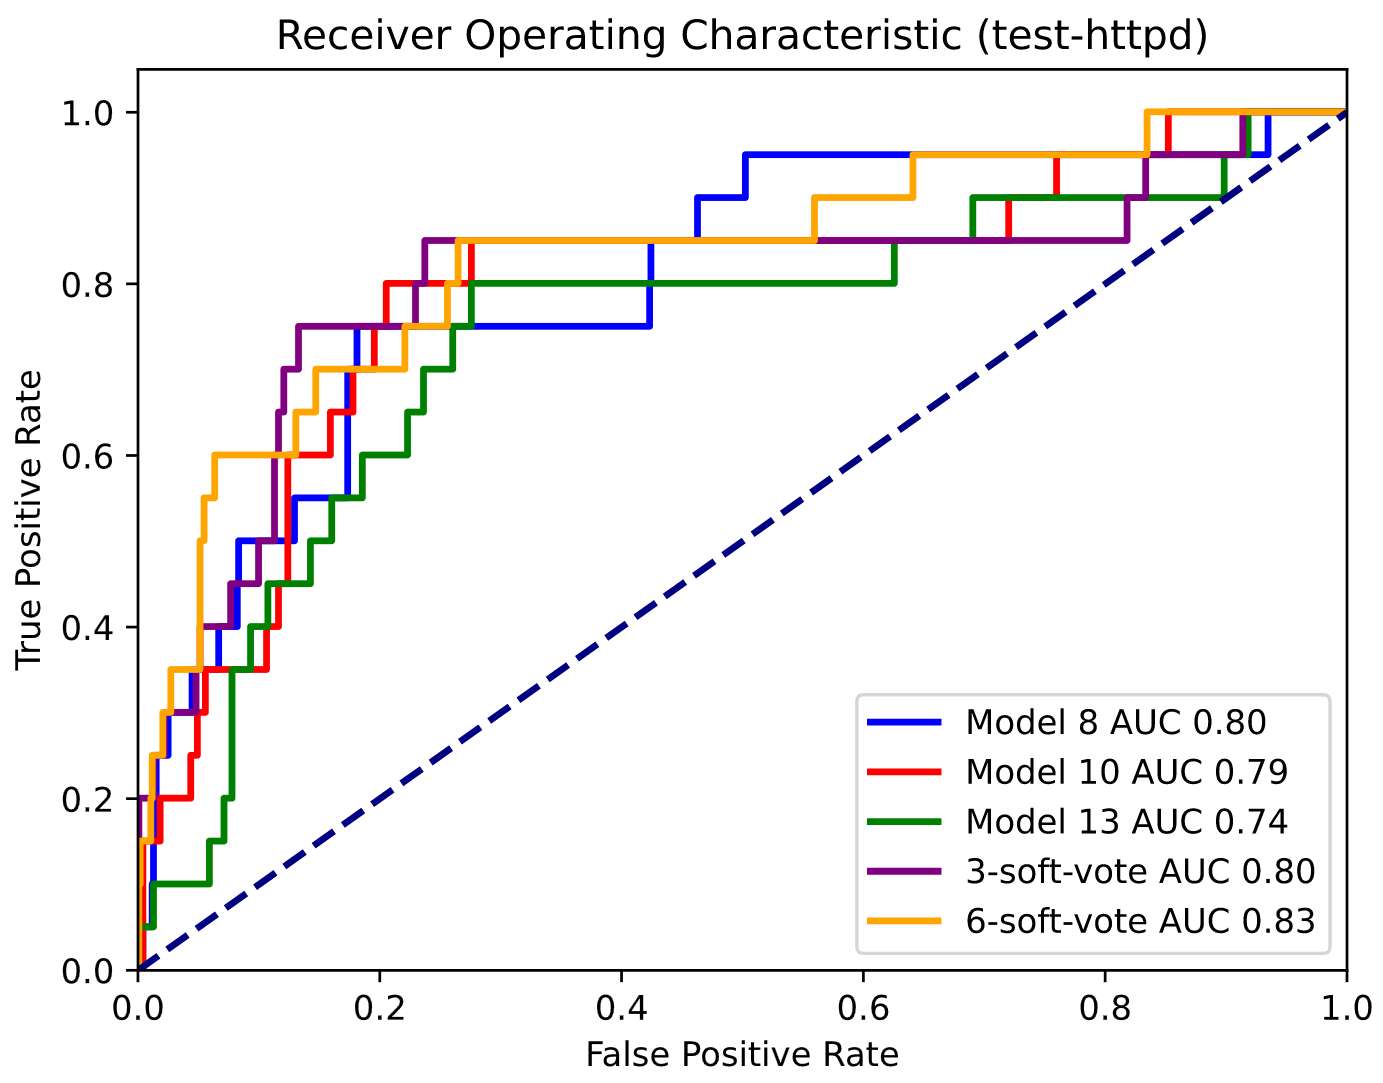
\includegraphics[width=0.75\textwidth]{figures/auc-httpd.png}
	\caption{The figure shows ROC curves for the top-performing models developed in this thesis. The models were evaluated on test data from the httpd project.}
	\label{figure:auc-httpd}
\end{figure}

\begin{figure}[ht]
	\centering
	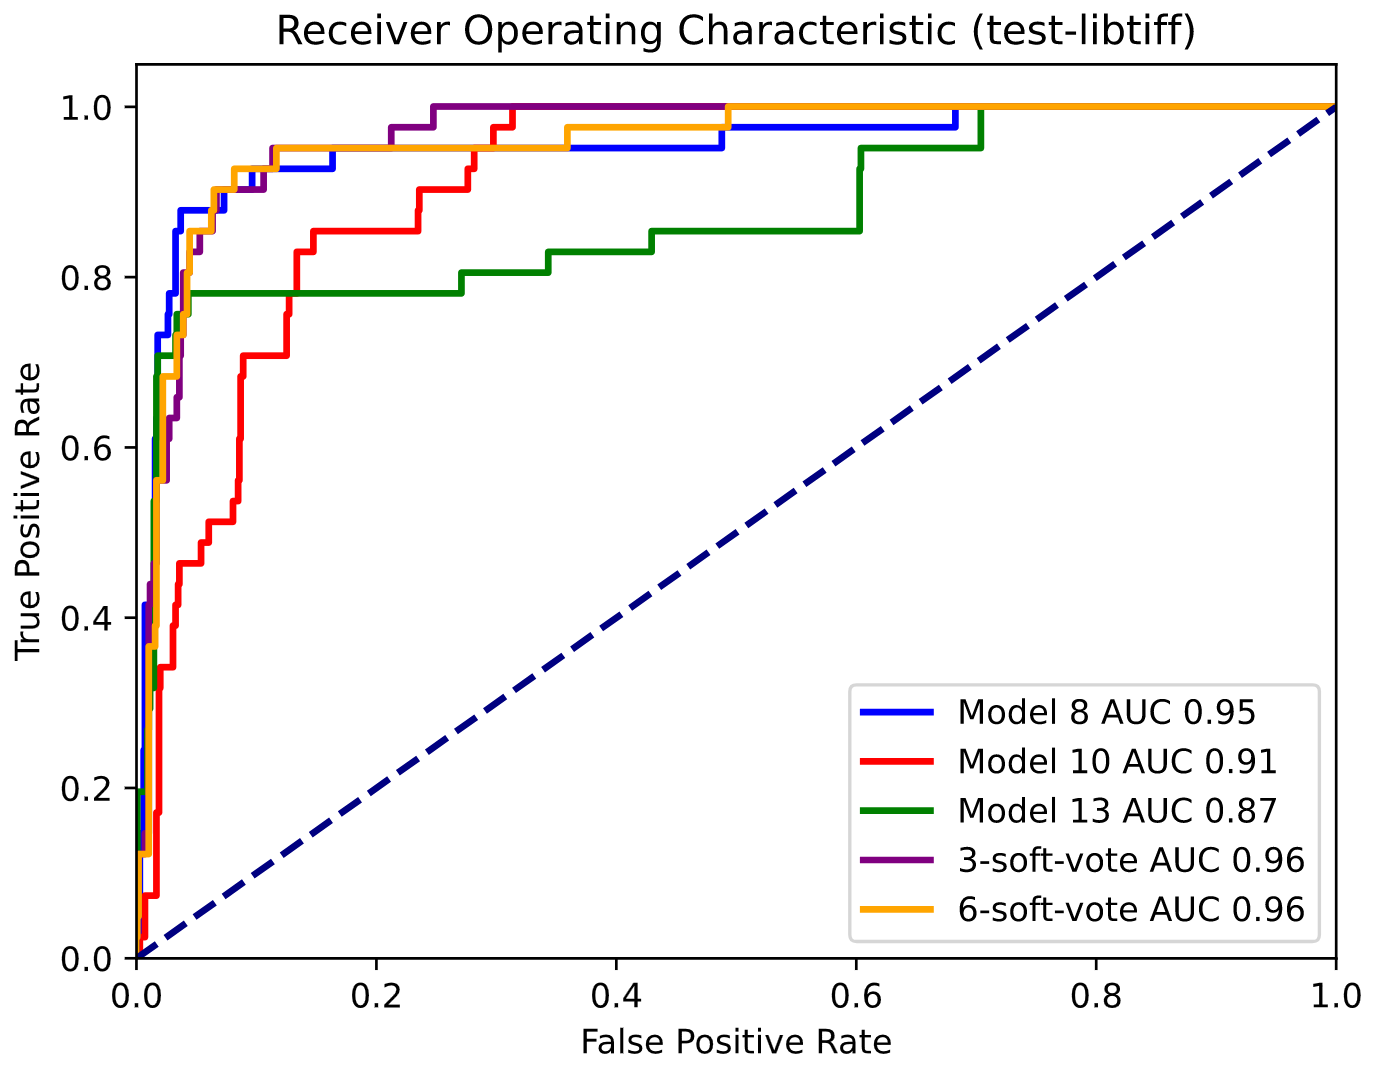
\includegraphics[width=0.75\textwidth]{figures/auc-libtiff.png}
	\caption{The figure shows ROC curves for the top-performing models developed in this thesis. The models were evaluated on test data from the libtiff project.}
	\label{figure:auc-libtiff}
\end{figure}

\begin{figure}[ht]
	\centering
	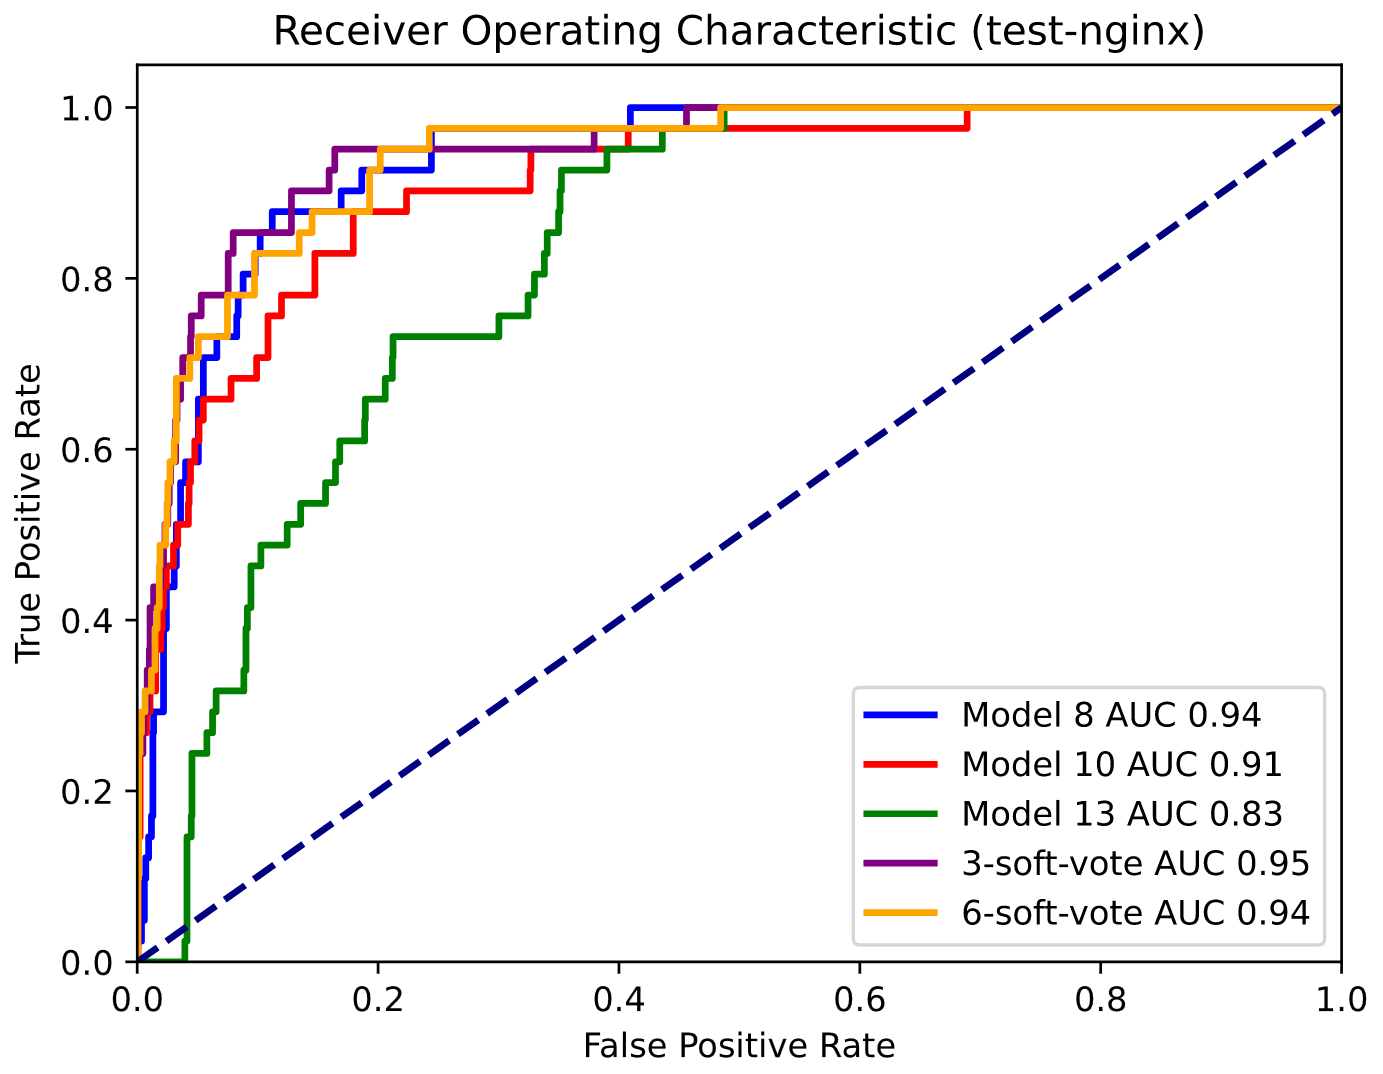
\includegraphics[width=0.75\textwidth]{figures/auc-nginx.png}
	\caption{The figure shows ROC curves for the top-performing models developed in this thesis. The models were evaluated on test data from the nginx project.}
	\label{figure:auc-nginx}
\end{figure}

\begin{figure}[ht]
	\centering
	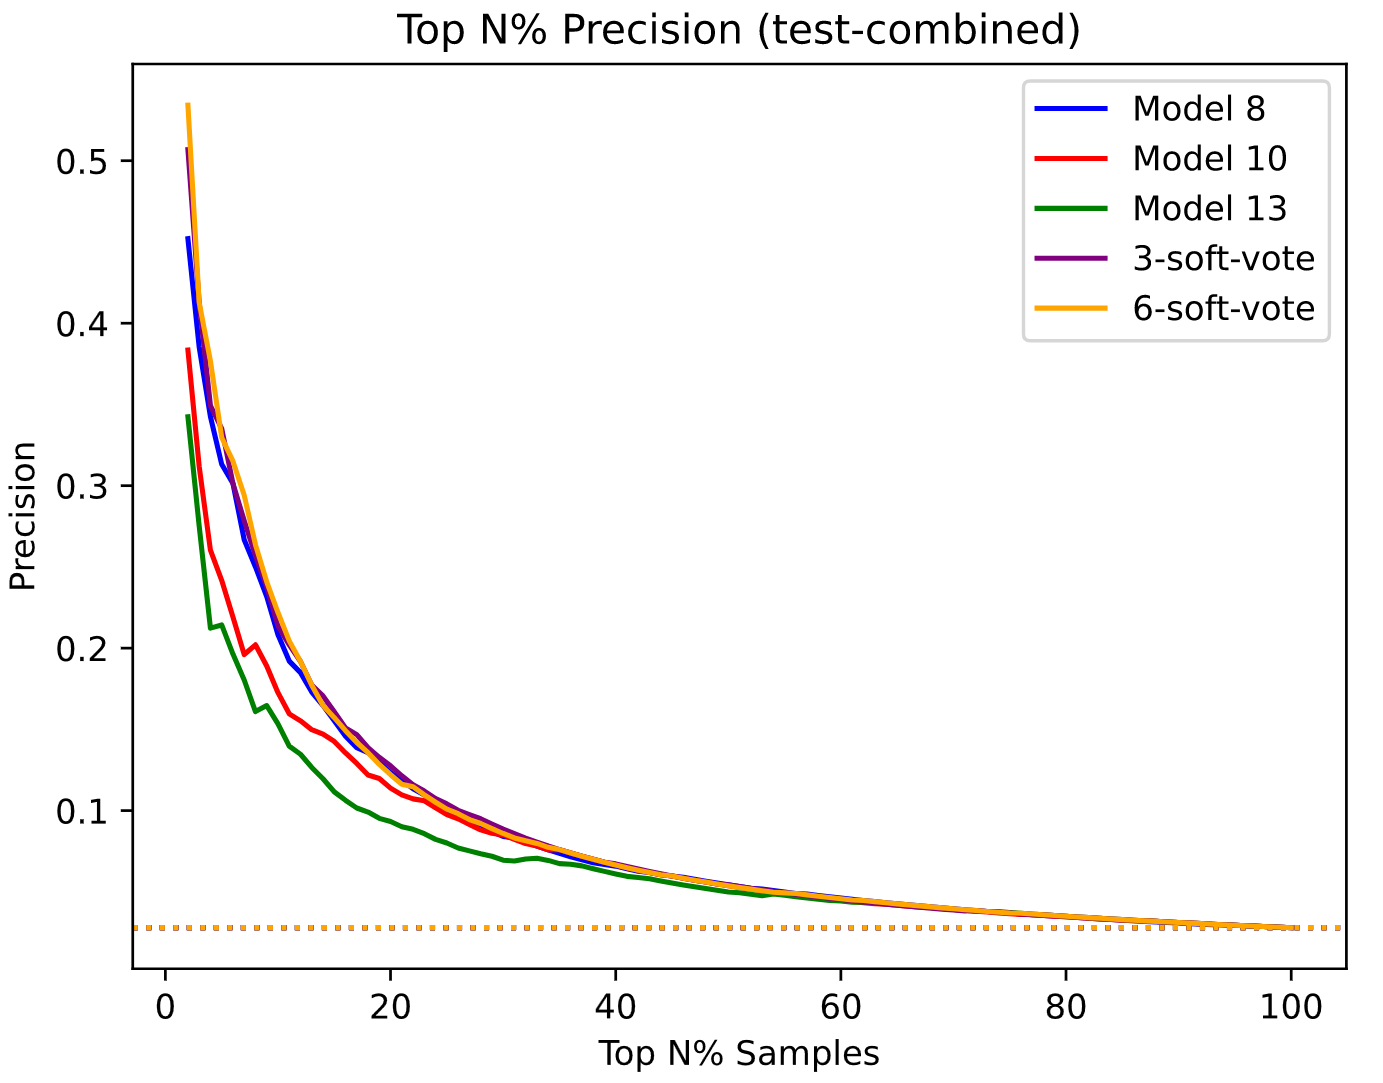
\includegraphics[width=0.75\textwidth]{figures/topn-combined.png}
	\caption{The figure shows the precision of top-performing models for various percentages of top-ranked samples. The models were evaluated on combined test data from the httpd, libtiff, and nginx projects. The dashed horizontal line indicates the precision of a random model.}
	\label{figure:topn-combined}
\end{figure}

\begin{figure}[ht]
	\centering
	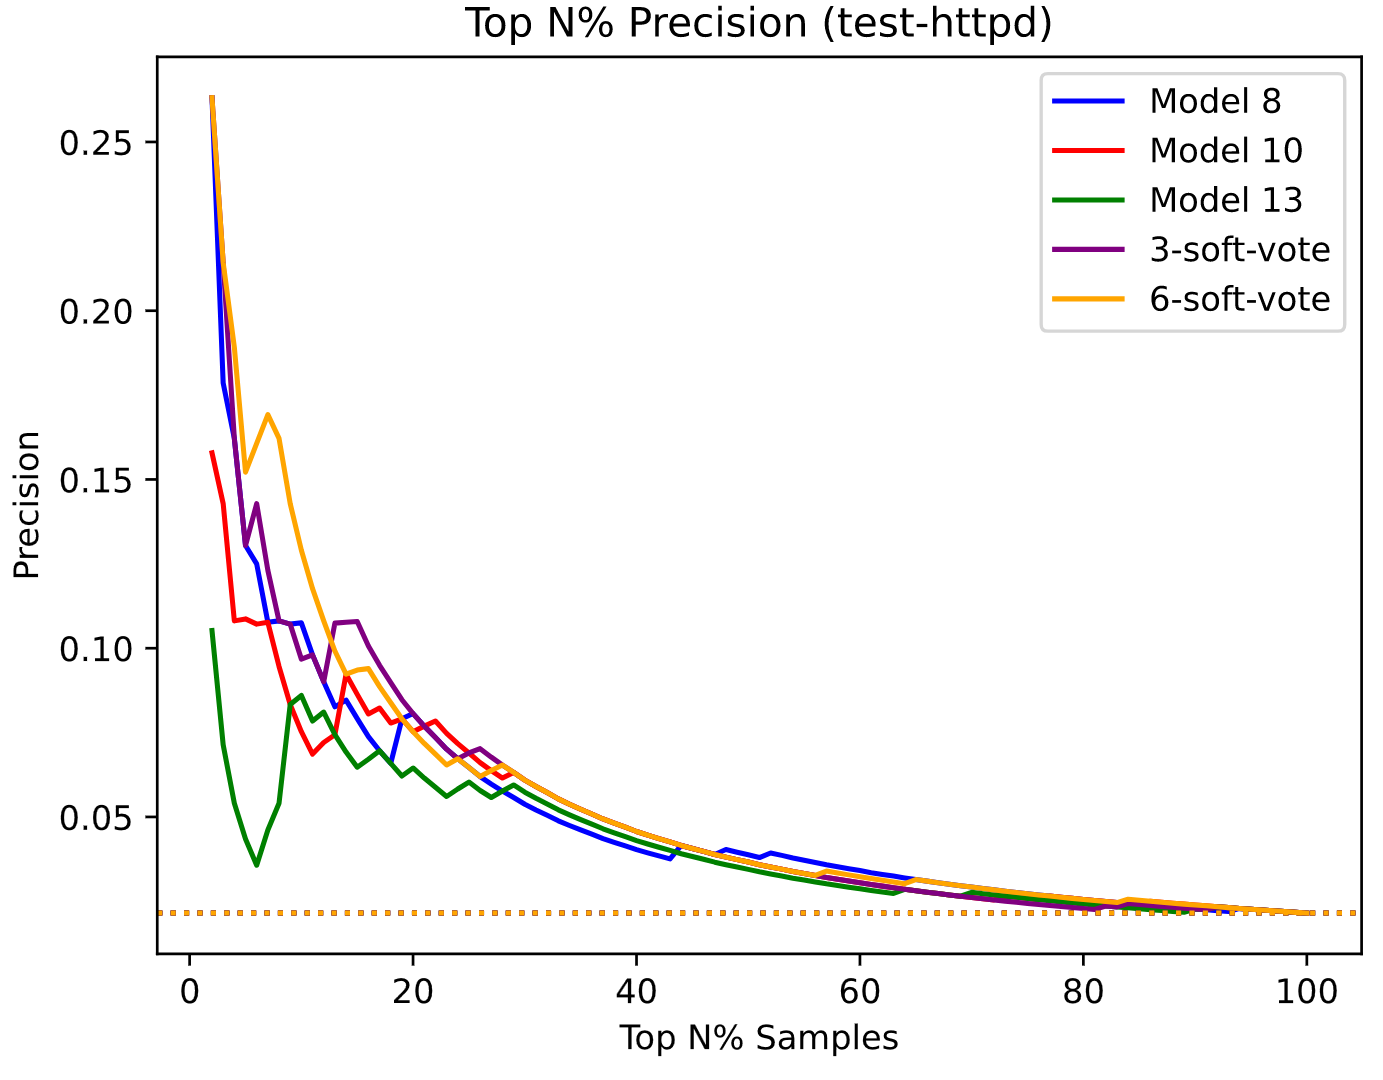
\includegraphics[width=0.75\textwidth]{figures/topn-httpd.png}
	\caption{The figure shows the precision of top-performing models for various percentages of top-ranked samples. The models were evaluated on test data from the httpd project. The dashed horizontal line indicates the precision of a random model.}
	\label{figure:topn-httpd}
\end{figure}

\begin{figure}[ht]
	\centering
	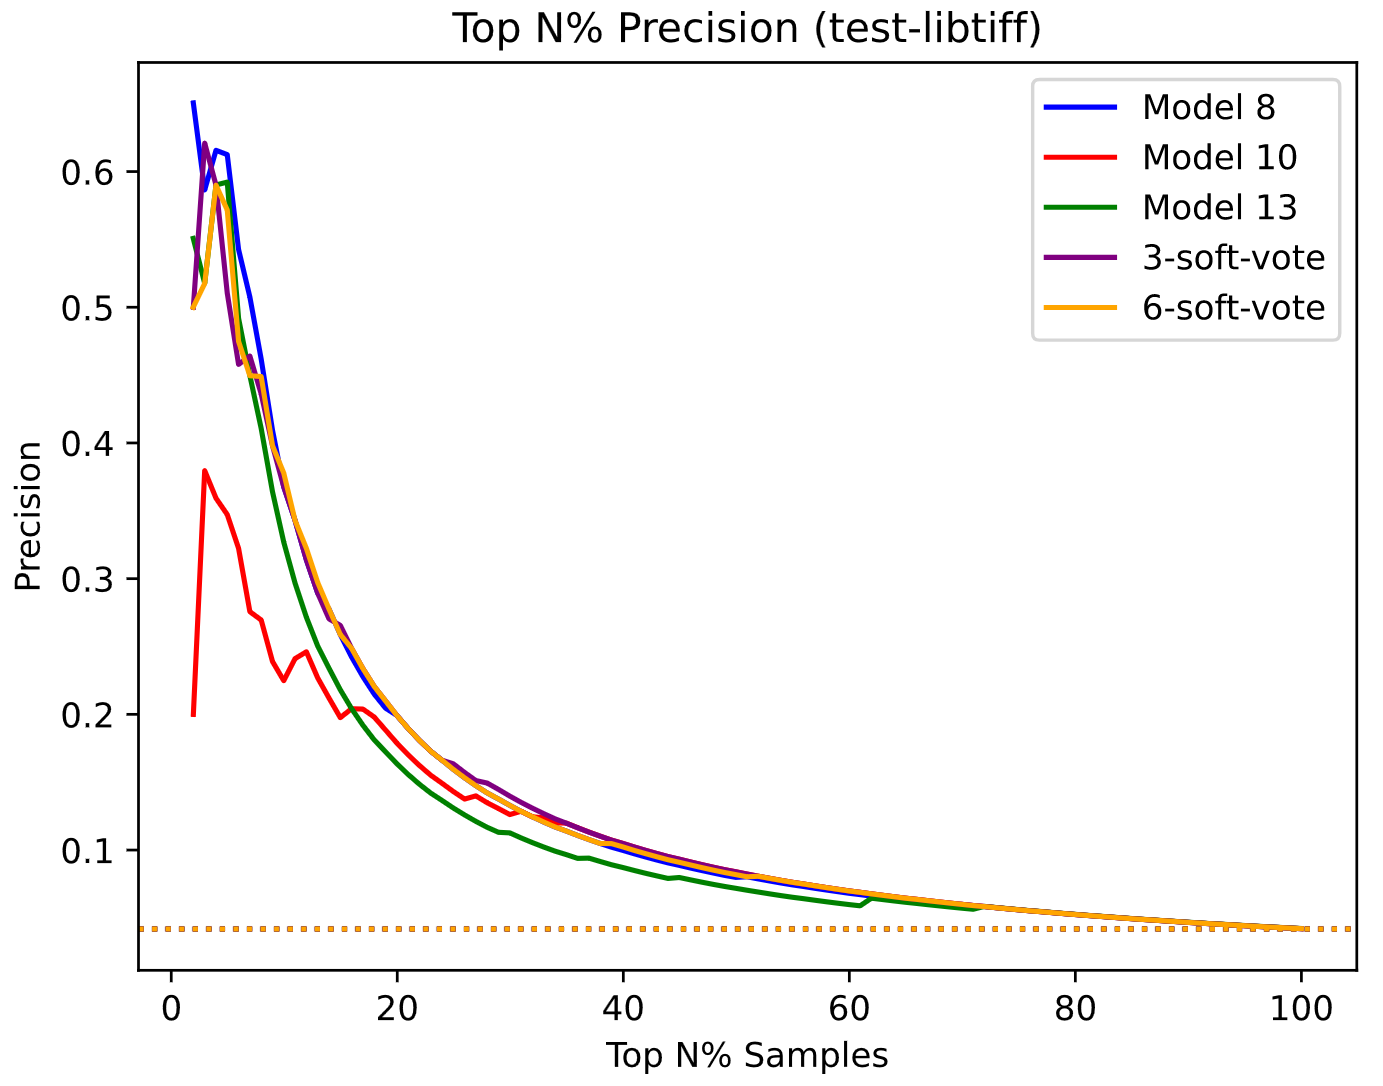
\includegraphics[width=0.75\textwidth]{figures/topn-libtiff.png}
	\caption{The figure shows the precision of top-performing models for various percentages of top-ranked samples. The models were evaluated on test data from the libtiff project. The dashed horizontal line indicates the precision of a random model.}
	\label{figure:topn-libtiff}
\end{figure}

\begin{figure}[ht]
	\centering
	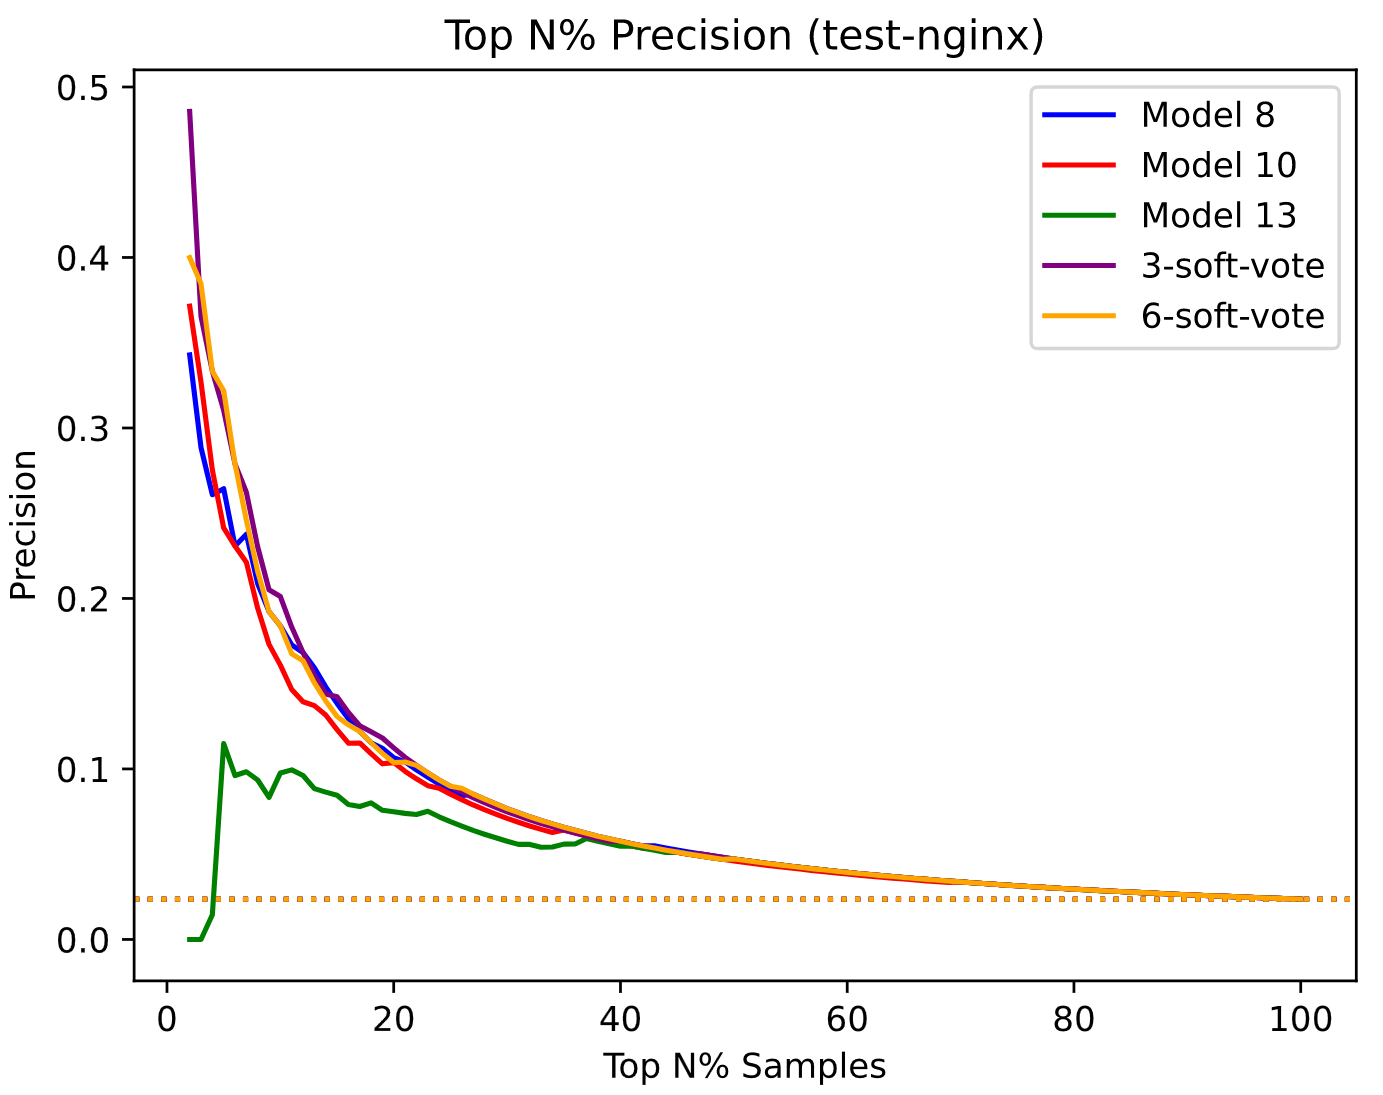
\includegraphics[width=0.75\textwidth]{figures/topn-nginx.png}
	\caption{The figure shows the precision of top-performing models for various percentages of top-ranked samples. The models were evaluated on test data from the nginx project. The dashed horizontal line indicates the precision of a random model.}
	\label{figure:topn-nginx}
\end{figure}


\begin{table}
    \centering
    \caption{The table shows all attributes for every node set present in Graph D2A. This table is divided into multiple parts by columns; this is Part 1. The remaining parts are in Tables~\ref{tab:attributes2},~\ref{tab:attributes3},~\ref{tab:attributes4},~\ref{tab:attributes5}, and~\ref{tab:attributes6}.}
    \vskip6pt
    \begin{tabular}{
        !{\vrule width 1pt}>{\centering\arraybackslash}m{1.95cm}!{\vrule width 1pt}
        >{\centering\arraybackslash}m{0.5cm}|
        >{\centering\arraybackslash}m{1cm}|
        >{\centering\arraybackslash}m{1.6cm}|
        >{\centering\arraybackslash}m{1cm}|
        >{\centering\arraybackslash}m{1.8cm}|
        >{\centering\arraybackslash}m{1.2cm}|
        >{\centering\arraybackslash}m{1cm}!{\vrule width 1pt}}
        
        \noalign{\hrule height 1pt}
        {\small Node Set} & {\scriptsize ID} & {\scriptsize LABEL} & {\scriptsize \hspace{0.2cm}LINE\newline NUMBER} & {\scriptsize CODE} & {\scriptsize \hspace{0.1cm}COLUMN\newline NUMBER} & {\scriptsize ORDER} & {\scriptsize NAME} \\
        \noalign{\hrule height 1pt}
        {\scriptsize META DATA}                                             & {\scriptsize \xmark} & {\scriptsize \xmark} & {\scriptsize -}         & {\scriptsize -} & {\scriptsize -} & {\scriptsize -} & {\scriptsize -}\\ \hline 
        {\scriptsize FILE}                                                  & {\scriptsize \xmark} & {\scriptsize \xmark} & {\scriptsize \xmark}    & {\scriptsize \xmark} & {\scriptsize \xmark} & {\scriptsize \xmark} & {\scriptsize \xmark}\\ \hline 
        {\scriptsize NAMESPACE}                                             & {\scriptsize \xmark} & {\scriptsize \xmark} & {\scriptsize \xmark}    & {\scriptsize \xmark} & {\scriptsize \xmark} & {\scriptsize \xmark} & {\scriptsize \xmark}\\ \hline 
        {\scriptsize NAMESPACE\newline BLOCK}                               & {\scriptsize \xmark} & {\scriptsize \xmark} & {\scriptsize \xmark}    & {\scriptsize \xmark} & {\scriptsize \xmark} & {\scriptsize \xmark} & {\scriptsize \xmark}\\ \hline 
        {\scriptsize METHOD}                                                & {\scriptsize \xmark} & {\scriptsize \checkmark} & {\scriptsize \xmark} & {\scriptsize \xmark} & {\scriptsize \xmark} & {\scriptsize \checkmark} & {\scriptsize \xmark}\\ \hline 
        {\scriptsize \hspace{0.02cm} METHOD\newline PARAMETER\newline IN}  & {\scriptsize \xmark} & {\scriptsize \checkmark} & {\scriptsize \xmark} & {\scriptsize \xmark} & {\scriptsize \xmark} & {\scriptsize \checkmark} & {\scriptsize \xmark}\\ \hline 
        {\scriptsize \hspace{0.02cm} METHOD\newline PARAMETER\newline OUT}   & {\scriptsize \xmark} & {\scriptsize \xmark} & {\scriptsize \xmark}    & {\scriptsize \xmark} & {\scriptsize \xmark} & {\scriptsize \xmark} & {\scriptsize \xmark}\\ \hline 
        {\scriptsize \hspace{0.02cm} METHOD\newline RETURN}                 & {\scriptsize \xmark} & {\scriptsize \checkmark} & {\scriptsize \xmark} & {\scriptsize \xmark} & {\scriptsize \xmark} & {\scriptsize \checkmark} & {\scriptsize -}\\ \hline 
        {\scriptsize MEMBER}                                                & {\scriptsize \xmark} & {\scriptsize \checkmark} & {\scriptsize \xmark} & {\scriptsize \xmark} & {\scriptsize \xmark} & {\scriptsize \checkmark} & {\scriptsize \xmark}\\ \hline 
        {\scriptsize TYPE}                                                  & {\scriptsize \xmark} & {\scriptsize \checkmark} & {\scriptsize -}     & {\scriptsize -} & {\scriptsize -} & {\scriptsize -} & {\scriptsize \xmark}\\ \hline 
        {\scriptsize TYPE DECL}                                             & {\scriptsize \xmark} & {\scriptsize \xmark} & {\scriptsize \xmark}    & {\scriptsize \xmark} & {\scriptsize \xmark} & {\scriptsize \xmark} & {\scriptsize \xmark}\\ \hline 
        {\scriptsize BLOCK}                                                 & {\scriptsize \xmark} & {\scriptsize \checkmark} & {\scriptsize \xmark} & {\scriptsize \xmark} & {\scriptsize \xmark} & {\scriptsize \checkmark} & {\scriptsize -}\\ \hline 
        {\scriptsize CALL}                                                  & {\scriptsize \xmark} & {\scriptsize \checkmark} & {\scriptsize \xmark} & {\scriptsize \xmark} & {\scriptsize \xmark} & {\scriptsize \checkmark} & {\scriptsize \xmark}\\ \hline 
        {\scriptsize \hspace{0.02cm} FIELD\newline IDENTIFIER}              & {\scriptsize \xmark} & {\scriptsize \checkmark} & {\scriptsize \xmark} & {\scriptsize \xmark} & {\scriptsize \xmark} & {\scriptsize \checkmark} & {\scriptsize -}\\ \hline 
        {\scriptsize IDENTIFIER}                                            & {\scriptsize \xmark} & {\scriptsize \checkmark} & {\scriptsize \xmark} & {\scriptsize \xmark} & {\scriptsize \xmark} & {\scriptsize \checkmark} & {\scriptsize \xmark}\\ \hline 
        {\scriptsize LITERAL}                                               & {\scriptsize \xmark} & {\scriptsize \checkmark} & {\scriptsize \xmark} & {\scriptsize \checkmark} & {\scriptsize \xmark} & {\scriptsize \checkmark} & {\scriptsize -}\\ \hline 
        {\scriptsize LOCAL}                                                 & {\scriptsize \xmark} & {\scriptsize \checkmark} & {\scriptsize \xmark} & {\scriptsize \xmark} & {\scriptsize \xmark} & {\scriptsize \checkmark} & {\scriptsize \xmark}\\ \hline 
        {\scriptsize \hspace{0.02cm} METHOD\newline REF}                    & {\scriptsize \xmark} & {\scriptsize \checkmark} & {\scriptsize \xmark} & {\scriptsize \xmark} & {\scriptsize \xmark} & {\scriptsize \checkmark} & {\scriptsize -}\\ \hline 
        {\scriptsize RETURN}                                                & {\scriptsize \xmark} & {\scriptsize \checkmark} & {\scriptsize \xmark} & {\scriptsize \xmark} & {\scriptsize \xmark} & {\scriptsize \checkmark} & {\scriptsize -}\\ \hline 
        {\scriptsize UNKNOWN}                                               & {\scriptsize \xmark} & {\scriptsize \checkmark} & {\scriptsize \xmark} & {\scriptsize \xmark} & {\scriptsize \xmark} & {\scriptsize \checkmark} & {\scriptsize -}\\ \hline 
        \noalign{\hrule height 1pt}
    \end{tabular}
    \label{tab:attributes1}
\end{table}










\begin{table}
    \centering
    \caption{The table shows all attributes for every node set present in Graph D2A. This table is divided into multiple parts by columns; this is Part 2. The remaining parts are in Tables~\ref{tab:attributes1},~\ref{tab:attributes3},~\ref{tab:attributes4},~\ref{tab:attributes5}, and~\ref{tab:attributes6}.}
    \vskip6pt
    \begin{tabular}{
        !{\vrule width 1pt}>{\centering\arraybackslash}m{1.95cm}!{\vrule width 1pt}
        >{\centering\arraybackslash}m{1.8cm}|
        >{\centering\arraybackslash}m{1.8cm}|
        >{\centering\arraybackslash}m{0.9cm}|
        >{\centering\arraybackslash}m{2.8cm}|
        >{\centering\arraybackslash}m{1.7cm}|
        >{\centering\arraybackslash}m{0.9cm}!{\vrule width 1pt}}
        
        \noalign{\hrule height 1pt}
        {\small Node Set} & {\scriptsize ARGUMENT \newline INDEX} & {\scriptsize ARGUMENT\newline NAME} & {\scriptsize TYPE\newline FULL\newline NAME} & {\scriptsize \hspace{0.1cm}DYNAMIC TYPE\newline HINT FULL NAME} & {\scriptsize FILENAME} & {\scriptsize \hspace{0.05cm}FULL\newline NAME} \\
        \noalign{\hrule height 1pt}
        {\scriptsize META DATA}                                             & {\scriptsize -} & {\scriptsize -} & {\scriptsize -} & {\scriptsize -} & {\scriptsize -} & {\scriptsize -} \\ \hline 
        {\scriptsize FILE}                                                  & {\scriptsize -} & {\scriptsize -} & {\scriptsize -} & {\scriptsize -} & {\scriptsize -} & {\scriptsize -} \\ \hline 
        {\scriptsize NAMESPACE}                                             & {\scriptsize -} & {\scriptsize -} & {\scriptsize -} & {\scriptsize -} & {\scriptsize -} & {\scriptsize -} \\ \hline 
        {\scriptsize NAMESPACE\newline BLOCK}                               & {\scriptsize -} & {\scriptsize -} & {\scriptsize -} & {\scriptsize -} & {\scriptsize \xmark} & {\scriptsize \xmark} \\ \hline 
        {\scriptsize METHOD}                                                & {\scriptsize -} & {\scriptsize -} & {\scriptsize -} & {\scriptsize -} & {\scriptsize \xmark} & {\scriptsize \checkmark} \\ \hline 
        {\scriptsize \hspace{0.02cm} METHOD\newline PARAMETER\newline IN}  & {\scriptsize -} & {\scriptsize -} & {\scriptsize \xmark} & {\scriptsize \xmark} & {\scriptsize -} & {\scriptsize -} \\ \hline 
        {\scriptsize \hspace{0.02cm} METHOD\newline PARAMETER\newline OUT}   & {\scriptsize -} & {\scriptsize -} & {\scriptsize \xmark} & {\scriptsize -} & {\scriptsize -} & {\scriptsize -} \\ \hline 
        {\scriptsize \hspace{0.02cm} METHOD\newline RETURN}                 & {\scriptsize -} & {\scriptsize -} & {\scriptsize \xmark} & {\scriptsize \xmark} & {\scriptsize -} & {\scriptsize -} \\ \hline 
        {\scriptsize MEMBER}                                                & {\scriptsize -} & {\scriptsize -} & {\scriptsize \xmark} & {\scriptsize \xmark} & {\scriptsize -} & {\scriptsize -} \\ \hline 
        {\scriptsize TYPE}                                                  & {\scriptsize -} & {\scriptsize -} & {\scriptsize -} & {\scriptsize -} & {\scriptsize -} & {\scriptsize \checkmark} \\ \hline 
        {\scriptsize TYPE DECL}                                             & {\scriptsize -} & {\scriptsize -} & {\scriptsize -} & {\scriptsize -} & {\scriptsize \xmark} & {\scriptsize \xmark} \\ \hline 
        {\scriptsize BLOCK}                                                 & {\scriptsize \checkmark} & {\scriptsize \xmark} & {\scriptsize \xmark} & {\scriptsize \xmark} & {\scriptsize -} & {\scriptsize -} \\ \hline 
        {\scriptsize CALL}                                                  & {\scriptsize \checkmark} & {\scriptsize \xmark} & {\scriptsize \xmark} & {\scriptsize \xmark} & {\scriptsize -} & {\scriptsize -} \\ \hline 
        {\scriptsize \hspace{0.02cm} FIELD\newline IDENTIFIER}              & {\scriptsize \checkmark} & {\scriptsize \xmark} & {\scriptsize -} & {\scriptsize -} & {\scriptsize -} & {\scriptsize -} \\ \hline 
        {\scriptsize IDENTIFIER}                                            & {\scriptsize \checkmark} & {\scriptsize \xmark} & {\scriptsize \xmark} & {\scriptsize \xmark} & {\scriptsize -} & {\scriptsize -} \\ \hline 
        {\scriptsize LITERAL}                                               & {\scriptsize \checkmark} & {\scriptsize \xmark} & {\scriptsize \xmark} & {\scriptsize \xmark} & {\scriptsize -} & {\scriptsize -} \\ \hline 
        {\scriptsize LOCAL}                                                 & {\scriptsize -} & {\scriptsize -} & {\scriptsize \xmark} & {\scriptsize \xmark} & {\scriptsize -} & {\scriptsize -} \\ \hline 
        {\scriptsize \hspace{0.02cm} METHOD\newline REF}                    & {\scriptsize \checkmark} & {\scriptsize \xmark} & {\scriptsize \xmark} & {\scriptsize \xmark} & {\scriptsize -} & {\scriptsize -} \\ \hline 
        {\scriptsize RETURN}                                                & {\scriptsize \checkmark} & {\scriptsize \xmark} & {\scriptsize -} & {\scriptsize -} & {\scriptsize -} & {\scriptsize -} \\ \hline 
        {\scriptsize UNKNOWN}                                               & {\scriptsize \checkmark} & {\scriptsize \xmark} & {\scriptsize \xmark} & {\scriptsize \xmark} & {\scriptsize -} & {\scriptsize -} \\ \hline 
        \noalign{\hrule height 1pt}
    \end{tabular}
    \label{tab:attributes2}
\end{table}

\begin{table}
    \centering
    \caption{The table shows all attributes for every node set present in Graph D2A. This table is divided into multiple parts by columns; this is Part 3. The remaining parts are in Tables~\ref{tab:attributes1},~\ref{tab:attributes2},~\ref{tab:attributes4},~\ref{tab:attributes5}, and~\ref{tab:attributes6}.}
    \vskip6pt
    \begin{tabular}{
        !{\vrule width 1pt}>{\centering\arraybackslash}m{1.95cm}!{\vrule width 1pt}
        >{\centering\arraybackslash}m{1.8cm}|
        >{\centering\arraybackslash}m{1.5cm}|
        >{\centering\arraybackslash}m{1.5cm}|
        >{\centering\arraybackslash}m{2cm}|
        >{\centering\arraybackslash}m{1cm}|
        >{\centering\arraybackslash}m{2.5cm}!{\vrule width 1pt}}
        
        \noalign{\hrule height 1pt}
        {\small Node Set} & {\scriptsize SIGNATURE} & {\scriptsize \hspace{0.05cm}METHOD\newline \hspace{0.1cm}FULL\newline NAME} & {\scriptsize \hspace{0.1cm}PARSER\newline TYPE\newline NAME} & {\scriptsize EVALUATION\newline STRATEGY} & {\scriptsize HASH} & {\scriptsize \hspace{0.15cm}AST PARENT \newline FULL NAME}\\
        \noalign{\hrule height 1pt}
        {\scriptsize META DATA}                                             & {\scriptsize -} & {\scriptsize -} & {\scriptsize -} & {\scriptsize -} & {\scriptsize \xmark} & {\scriptsize -} \\ \hline 
        {\scriptsize FILE}                                                  & {\scriptsize -} & {\scriptsize -} & {\scriptsize -} & {\scriptsize -} & {\scriptsize \xmark} & {\scriptsize -} \\ \hline 
        {\scriptsize NAMESPACE}                                             & {\scriptsize -} & {\scriptsize -} & {\scriptsize -} & {\scriptsize -} & {\scriptsize -} & {\scriptsize -} \\ \hline 
        {\scriptsize NAMESPACE\newline BLOCK}                               & {\scriptsize -} & {\scriptsize -} & {\scriptsize -} & {\scriptsize -} & {\scriptsize -} & {\scriptsize -} \\ \hline 
        {\scriptsize METHOD}                                                & {\scriptsize \xmark} & {\scriptsize -} & {\scriptsize -} & {\scriptsize -} & {\scriptsize \xmark} & {\scriptsize \xmark} \\ \hline 
        {\scriptsize \hspace{0.02cm} METHOD\newline PARAMETER\newline IN}  & {\scriptsize -} & {\scriptsize -} & {\scriptsize -} & {\scriptsize \xmark} & {\scriptsize -} & {\scriptsize -} \\ \hline 
        {\scriptsize \hspace{0.02cm} METHOD\newline PARAMETER\newline OUT}   & {\scriptsize -} & {\scriptsize -} & {\scriptsize -} & {\scriptsize \xmark} & {\scriptsize -} & {\scriptsize -} \\ \hline 
        {\scriptsize \hspace{0.02cm} METHOD\newline RETURN}                 & {\scriptsize -} & {\scriptsize -} & {\scriptsize -} & {\scriptsize \xmark} & {\scriptsize -} & {\scriptsize -} \\ \hline 
        {\scriptsize MEMBER}                                                & {\scriptsize -} & {\scriptsize -} & {\scriptsize -} & {\scriptsize -} & {\scriptsize -} & {\scriptsize -} \\ \hline 
        {\scriptsize TYPE}                                                  & {\scriptsize -} & {\scriptsize -} & {\scriptsize -} & {\scriptsize -} & {\scriptsize -} & {\scriptsize -} \\ \hline 
        {\scriptsize TYPE DECL}                                             & {\scriptsize -} & {\scriptsize -} & {\scriptsize -} & {\scriptsize -} & {\scriptsize -} & {\scriptsize \xmark} \\ \hline 
        {\scriptsize BLOCK}                                                 & {\scriptsize -} & {\scriptsize -} & {\scriptsize -} & {\scriptsize -} & {\scriptsize -} & {\scriptsize -} \\ \hline 
        {\scriptsize CALL}                                                  & {\scriptsize \xmark} & {\scriptsize \xmark} & {\scriptsize -} & {\scriptsize -} & {\scriptsize -} & {\scriptsize -} \\ \hline 
        {\scriptsize \hspace{0.02cm} FIELD\newline IDENTIFIER}              & {\scriptsize -} & {\scriptsize -} & {\scriptsize -} & {\scriptsize -} & {\scriptsize -} & {\scriptsize -} \\ \hline 
        {\scriptsize IDENTIFIER}                                            & {\scriptsize -} & {\scriptsize -} & {\scriptsize -} & {\scriptsize -} & {\scriptsize -} & {\scriptsize -} \\ \hline 
        {\scriptsize LITERAL}                                               & {\scriptsize -} & {\scriptsize -} & {\scriptsize -} & {\scriptsize -} & {\scriptsize -} & {\scriptsize -} \\ \hline 
        {\scriptsize LOCAL}                                                 & {\scriptsize -} & {\scriptsize -} & {\scriptsize -} & {\scriptsize -} & {\scriptsize -} & {\scriptsize -} \\ \hline 
        {\scriptsize \hspace{0.02cm} METHOD\newline REF}                    & {\scriptsize -} & {\scriptsize \xmark} & {\scriptsize -} & {\scriptsize -} & {\scriptsize -} & {\scriptsize -} \\ \hline 
        {\scriptsize RETURN}                                                & {\scriptsize -} & {\scriptsize -} & {\scriptsize -} & {\scriptsize -} & {\scriptsize -} & {\scriptsize -} \\ \hline 
        {\scriptsize UNKNOWN}                                               & {\scriptsize -} & {\scriptsize -} & {\scriptsize \xmark} & {\scriptsize -} & {\scriptsize -} & {\scriptsize -} \\ \hline 
        \noalign{\hrule height 1pt}
    \end{tabular}
    \label{tab:attributes3}
\end{table}


\begin{table}
    \centering
    \caption{The table shows all attributes for every node set present in Graph D2A. This table is divided into multiple parts by columns; this is Part 4. The remaining parts are in Tables~\ref{tab:attributes1},~\ref{tab:attributes2},~\ref{tab:attributes3},~\ref{tab:attributes5}, and~\ref{tab:attributes6}.}
    \vskip6pt
    \begin{tabular}{
        !{\vrule width 1pt}>{\centering\arraybackslash}m{1.95cm}!{\vrule width 1pt}
        >{\centering\arraybackslash}m{1.2cm}|
        >{\centering\arraybackslash}m{1.8cm}|
        >{\centering\arraybackslash}m{1.1cm}|
        >{\centering\arraybackslash}m{1.6cm}|
        >{\centering\arraybackslash}m{1.4cm}|
        >{\centering\arraybackslash}m{1.6cm}!{\vrule width 1pt}}
        
        \noalign{\hrule height 1pt}
        {\small Node Set} & {\scriptsize \hspace{0.1cm}AST\newline PARENT\newline TYPE} & {\scriptsize \hspace{0.3cm}IS\newline EXTERNAL} & {\scriptsize INDEX} & {\scriptsize \hspace{0.3cm}IS\newline VARIADIC} & {\scriptsize COLUMN\newline NUMBER\newline END} & {\scriptsize \hspace{0.2cm}LINE\newline NUMBER\newline END}\\
        \noalign{\hrule height 1pt}
        {\scriptsize META DATA}                                             & {\scriptsize -} & {\scriptsize -} & {\scriptsize -} & {\scriptsize -} & {\scriptsize -} & {\scriptsize -} \\ \hline 
        {\scriptsize FILE}                                                  & {\scriptsize -} & {\scriptsize -} & {\scriptsize -} & {\scriptsize -} & {\scriptsize -} & {\scriptsize -} \\ \hline 
        {\scriptsize NAMESPACE}                                             & {\scriptsize -} & {\scriptsize -} & {\scriptsize -} & {\scriptsize -} & {\scriptsize -} & {\scriptsize -} \\ \hline 
        {\scriptsize NAMESPACE\newline BLOCK}                               & {\scriptsize -} & {\scriptsize -} & {\scriptsize -} & {\scriptsize -} & {\scriptsize -} & {\scriptsize -} \\ \hline 
        {\scriptsize METHOD}                                                & {\scriptsize \xmark} & {\scriptsize \checkmark} & {\scriptsize -} & {\scriptsize -} & {\scriptsize \xmark} & {\scriptsize \xmark} \\ \hline 
        {\scriptsize \hspace{0.02cm} METHOD\newline PARAMETER\newline IN}  & {\scriptsize -} & {\scriptsize -} & {\scriptsize \xmark} & {\scriptsize \xmark} & {\scriptsize -} & {\scriptsize -} \\ \hline 
        {\scriptsize \hspace{0.02cm} METHOD\newline PARAMETER\newline OUT}   & {\scriptsize -} & {\scriptsize -} & {\scriptsize \xmark} & {\scriptsize \xmark} & {\scriptsize -} & {\scriptsize -} \\ \hline 
        {\scriptsize \hspace{0.02cm} METHOD\newline RETURN}                 & {\scriptsize -} & {\scriptsize -} & {\scriptsize -} & {\scriptsize -} & {\scriptsize -} & {\scriptsize -} \\ \hline 
        {\scriptsize MEMBER}                                                & {\scriptsize -} & {\scriptsize -} & {\scriptsize -} & {\scriptsize -} & {\scriptsize -} & {\scriptsize -} \\ \hline 
        {\scriptsize TYPE}                                                  & {\scriptsize -} & {\scriptsize -} & {\scriptsize -} & {\scriptsize -} & {\scriptsize -} & {\scriptsize -} \\ \hline 
        {\scriptsize TYPE DECL}                                             & {\scriptsize \xmark} & {\scriptsize \xmark} & {\scriptsize -} & {\scriptsize -} & {\scriptsize -} & {\scriptsize -} \\ \hline 
        {\scriptsize BLOCK}                                                 & {\scriptsize -} & {\scriptsize -} & {\scriptsize -} & {\scriptsize -} & {\scriptsize -} & {\scriptsize -} \\ \hline 
        {\scriptsize CALL}                                                  & {\scriptsize -} & {\scriptsize -} & {\scriptsize -} & {\scriptsize -} & {\scriptsize -} & {\scriptsize -} \\ \hline 
        {\scriptsize \hspace{0.02cm} FIELD\newline IDENTIFIER}              & {\scriptsize -} & {\scriptsize -} & {\scriptsize -} & {\scriptsize -} & {\scriptsize -} & {\scriptsize -} \\ \hline 
        {\scriptsize IDENTIFIER}                                            & {\scriptsize -} & {\scriptsize -} & {\scriptsize -} & {\scriptsize -} & {\scriptsize -} & {\scriptsize -} \\ \hline 
        {\scriptsize LITERAL}                                               & {\scriptsize -} & {\scriptsize -} & {\scriptsize -} & {\scriptsize -} & {\scriptsize -} & {\scriptsize -} \\ \hline 
        {\scriptsize LOCAL}                                                 & {\scriptsize -} & {\scriptsize -} & {\scriptsize -} & {\scriptsize -} & {\scriptsize -} & {\scriptsize -} \\ \hline 
        {\scriptsize \hspace{0.02cm} METHOD\newline REF}                    & {\scriptsize -} & {\scriptsize -} & {\scriptsize -} & {\scriptsize -} & {\scriptsize -} & {\scriptsize -} \\ \hline 
        {\scriptsize RETURN}                                                & {\scriptsize -} & {\scriptsize -} & {\scriptsize -} & {\scriptsize -} & {\scriptsize -} & {\scriptsize -} \\ \hline 
        {\scriptsize UNKNOWN}                                               & {\scriptsize -} & {\scriptsize -} & {\scriptsize -} & {\scriptsize -} & {\scriptsize -} & {\scriptsize -} \\ \hline 
        \noalign{\hrule height 1pt}
    \end{tabular}
    \label{tab:attributes4}
\end{table}


\begin{table}
    \centering
    \caption{The table shows all attributes for every node set present in Graph D2A. This table is divided into multiple parts by columns; this is Part 5. The remaining parts are in Tables~\ref{tab:attributes1},~\ref{tab:attributes2},~\ref{tab:attributes3},~\ref{tab:attributes4}, and~\ref{tab:attributes6}.}
    \vskip6pt
    \begin{tabular}{
        !{\vrule width 1pt}>{\centering\arraybackslash}m{1.95cm}!{\vrule width 1pt}
        >{\centering\arraybackslash}m{1cm}|
        >{\centering\arraybackslash}m{1cm}|
        >{\centering\arraybackslash}m{1.8cm}|
        >{\centering\arraybackslash}m{1.5cm}|
        >{\centering\arraybackslash}m{1.9cm}|
        >{\centering\arraybackslash}m{1.5cm}!{\vrule width 1pt}}
        
        \noalign{\hrule height 1pt}
        {\small Node Set} & {\scriptsize TYPE\newline DECL\newline FULL\newline NAME} & {\scriptsize ALIAS\newline TYPE\newline FULL\newline NAME} & {\scriptsize CONTAINED\newline REF} & {\scriptsize CLOSURE\newline BINDING\newline ID} & {\scriptsize CANONICAL\newline NAME} & {\scriptsize DISPATCH\newline TYPE}\\
        \noalign{\hrule height 1pt}
        {\scriptsize META DATA}                                             & {\scriptsize -} & {\scriptsize -} & {\scriptsize -} & {\scriptsize -} & {\scriptsize -} & {\scriptsize -} \\ \hline 
        {\scriptsize FILE}                                                  & {\scriptsize -} & {\scriptsize -} & {\scriptsize -} & {\scriptsize -} & {\scriptsize -} & {\scriptsize -} \\ \hline 
        {\scriptsize NAMESPACE}                                             & {\scriptsize -} & {\scriptsize -} & {\scriptsize -} & {\scriptsize -} & {\scriptsize -} & {\scriptsize -} \\ \hline 
        {\scriptsize NAMESPACE\newline BLOCK}                               & {\scriptsize -} & {\scriptsize -} & {\scriptsize -} & {\scriptsize -} & {\scriptsize -} & {\scriptsize -} \\ \hline 
        {\scriptsize METHOD}                                                & {\scriptsize -} & {\scriptsize -} & {\scriptsize -} & {\scriptsize -} & {\scriptsize -} & {\scriptsize -} \\ \hline 
        {\scriptsize \hspace{0.02cm} METHOD\newline PARAMETER\newline IN}  & {\scriptsize -} & {\scriptsize -} & {\scriptsize -} & {\scriptsize -} & {\scriptsize -} & {\scriptsize -} \\ \hline 
        {\scriptsize \hspace{0.02cm} METHOD\newline PARAMETER\newline OUT}   & {\scriptsize -} & {\scriptsize -} & {\scriptsize -} & {\scriptsize -} & {\scriptsize -} & {\scriptsize -} \\ \hline 
        {\scriptsize \hspace{0.02cm} METHOD\newline RETURN}                 & {\scriptsize -} & {\scriptsize -} & {\scriptsize -} & {\scriptsize -} & {\scriptsize -} & {\scriptsize -} \\ \hline 
        {\scriptsize MEMBER}                                                & {\scriptsize -} & {\scriptsize -} & {\scriptsize -} & {\scriptsize -} & {\scriptsize -} & {\scriptsize -} \\ \hline 
        {\scriptsize TYPE}                                                  & {\scriptsize \xmark} & {\scriptsize -} & {\scriptsize -} & {\scriptsize -} & {\scriptsize -} & {\scriptsize -} \\ \hline 
        {\scriptsize TYPE DECL}                                             & {\scriptsize -} & {\scriptsize \xmark} & {\scriptsize -} & {\scriptsize -} & {\scriptsize -} & {\scriptsize -} \\ \hline 
        {\scriptsize BLOCK}                                                 & {\scriptsize -} & {\scriptsize -} & {\scriptsize -} & {\scriptsize -} & {\scriptsize -} & {\scriptsize -} \\ \hline 
        {\scriptsize CALL}                                                  & {\scriptsize -} & {\scriptsize -} & {\scriptsize -} & {\scriptsize -} & {\scriptsize -} & {\scriptsize \xmark} \\ \hline 
        {\scriptsize \hspace{0.02cm} FIELD\newline IDENTIFIER}              & {\scriptsize -} & {\scriptsize -} & {\scriptsize -} & {\scriptsize -} & {\scriptsize \xmark} & {\scriptsize -} \\ \hline 
        {\scriptsize IDENTIFIER}                                            & {\scriptsize -} & {\scriptsize -} & {\scriptsize -} & {\scriptsize -} & {\scriptsize -} & {\scriptsize -} \\ \hline 
        {\scriptsize LITERAL}                                               & {\scriptsize -} & {\scriptsize -} & {\scriptsize -} & {\scriptsize -} & {\scriptsize -} & {\scriptsize -} \\ \hline 
        {\scriptsize LOCAL}                                                 & {\scriptsize -} & {\scriptsize -} & {\scriptsize -} & {\scriptsize \xmark} & {\scriptsize -} & {\scriptsize -} \\ \hline 
        {\scriptsize \hspace{0.02cm} METHOD\newline REF}                    & {\scriptsize -} & {\scriptsize -} & {\scriptsize -} & {\scriptsize -} & {\scriptsize -} & {\scriptsize -} \\ \hline 
        {\scriptsize RETURN}                                                & {\scriptsize -} & {\scriptsize -} & {\scriptsize -} & {\scriptsize -} & {\scriptsize -} & {\scriptsize -} \\ \hline 
        {\scriptsize UNKNOWN}                                               & {\scriptsize -} & {\scriptsize -} & {\scriptsize \xmark} & {\scriptsize -} & {\scriptsize -} & {\scriptsize -} \\ \hline 
        \noalign{\hrule height 1pt}
    \end{tabular}
    \label{tab:attributes5}
\end{table}

\begin{table}
    \centering
    \caption{The table shows all attributes for every node set present in Graph D2A. This table is divided into multiple parts by columns; this is Part 1. The remaining parts are in Tables~\ref{tab:attributes1},~\ref{tab:attributes2},~\ref{tab:attributes3},~\ref{tab:attributes4}, and~\ref{tab:attributes5}.}
    \vskip6pt
    \begin{tabular}{
        !{\vrule width 1pt}>{\centering\arraybackslash}m{1.95cm}!{\vrule width 1pt}
        >{\centering\arraybackslash}m{1.8cm}|
        >{\centering\arraybackslash}m{1.8cm}|
        >{\centering\arraybackslash}m{1cm}|
        >{\centering\arraybackslash}m{1.4cm}|
        >{\centering\arraybackslash}m{3cm}!{\vrule width 1pt}}
        
        \noalign{\hrule height 1pt}
        {\small Node Set} & {\scriptsize LANGUAGE} & {\scriptsize OVERLAYS} & {\scriptsize ROOT} & {\scriptsize VERSION} & {\scriptsize \hspace{0.1cm}INHERITS FROM\newline TYPE FULL NAME}\\
        \noalign{\hrule height 1pt}
        {\scriptsize META DATA}                                             & {\scriptsize \xmark} & {\scriptsize \xmark} & {\scriptsize \xmark} & {\scriptsize \xmark} & {\scriptsize -} \\ \hline 
        {\scriptsize FILE}                                                  & {\scriptsize -} & {\scriptsize -} & {\scriptsize -} & {\scriptsize -} & {\scriptsize -} \\ \hline 
        {\scriptsize NAMESPACE}                                             & {\scriptsize -} & {\scriptsize -} & {\scriptsize -} & {\scriptsize -} & {\scriptsize -} \\ \hline 
        {\scriptsize NAMESPACE\newline BLOCK}                               & {\scriptsize -} & {\scriptsize -} & {\scriptsize -} & {\scriptsize -} & {\scriptsize -} \\ \hline 
        {\scriptsize METHOD}                                                & {\scriptsize -} & {\scriptsize -} & {\scriptsize -} & {\scriptsize -} & {\scriptsize -} \\ \hline 
        {\scriptsize \hspace{0.02cm} METHOD\newline PARAMETER\newline IN}  & {\scriptsize -} & {\scriptsize -} & {\scriptsize -} & {\scriptsize -} & {\scriptsize -} \\ \hline 
        {\scriptsize \hspace{0.02cm} METHOD\newline PARAMETER\newline OUT}   & {\scriptsize -} & {\scriptsize -} & {\scriptsize -} & {\scriptsize -} & {\scriptsize -} \\ \hline 
        {\scriptsize \hspace{0.02cm} METHOD\newline RETURN}                 & {\scriptsize -} & {\scriptsize -} & {\scriptsize -} & {\scriptsize -} & {\scriptsize -} \\ \hline 
        {\scriptsize MEMBER}                                                & {\scriptsize -} & {\scriptsize -} & {\scriptsize -} & {\scriptsize -} & {\scriptsize -} \\ \hline 
        {\scriptsize TYPE}                                                  & {\scriptsize -} & {\scriptsize -} & {\scriptsize -} & {\scriptsize -} & {\scriptsize -} \\ \hline 
        {\scriptsize TYPE DECL}                                             & {\scriptsize -} & {\scriptsize -} & {\scriptsize -} & {\scriptsize -} & {\scriptsize \xmark} \\ \hline 
        {\scriptsize BLOCK}                                                 & {\scriptsize -} & {\scriptsize -} & {\scriptsize -} & {\scriptsize -} & {\scriptsize -} \\ \hline 
        {\scriptsize CALL}                                                  & {\scriptsize -} & {\scriptsize -} & {\scriptsize -} & {\scriptsize -} & {\scriptsize -} \\ \hline 
        {\scriptsize \hspace{0.02cm} FIELD\newline IDENTIFIER}              & {\scriptsize -} & {\scriptsize -} & {\scriptsize -} & {\scriptsize -} & {\scriptsize -} \\ \hline 
        {\scriptsize IDENTIFIER}                                            & {\scriptsize -} & {\scriptsize -} & {\scriptsize -} & {\scriptsize -} & {\scriptsize -} \\ \hline 
        {\scriptsize LITERAL}                                               & {\scriptsize -} & {\scriptsize -} & {\scriptsize -} & {\scriptsize -} & {\scriptsize -} \\ \hline 
        {\scriptsize LOCAL}                                                 & {\scriptsize -} & {\scriptsize -} & {\scriptsize -} & {\scriptsize -} & {\scriptsize -} \\ \hline 
        {\scriptsize \hspace{0.02cm} METHOD\newline REF}                    & {\scriptsize -} & {\scriptsize -} & {\scriptsize -} & {\scriptsize -} & {\scriptsize -} \\ \hline 
        {\scriptsize RETURN}                                                & {\scriptsize -} & {\scriptsize -} & {\scriptsize -} & {\scriptsize -} & {\scriptsize -} \\ \hline 
        {\scriptsize UNKNOWN}                                               & {\scriptsize -} & {\scriptsize -} & {\scriptsize -} & {\scriptsize -} & {\scriptsize -} \\ \hline 
        \noalign{\hrule height 1pt}
    \end{tabular}
    \label{tab:attributes6}
\end{table}